\documentclass[journal]{IEEEtran}

% ---------------------------------------------------------------------------
% Preamble: identical packages to main.tex; graphics path points at paper/figures/
% (the post-E0.5 figures; legacy and retired figures are in figures/legacy and
% figures/retired). main.tex is untouched; this file assembles the new sections.
% ---------------------------------------------------------------------------

\usepackage{graphicx}
\usepackage{booktabs}
\usepackage{tabularx}
\usepackage{subfig}          % NOT subfigure or subcaption -- pick one, this is it
\usepackage{amsmath}
\usepackage{amssymb}
\usepackage{url}
\usepackage{xcolor}

\graphicspath{{figures/}}

\begin{document}

% Title and abstract come from abstract_title.tex (author's file, included unedited).
% IEEEtran needs \title before \maketitle and the abstract after it, so the file is input twice:
% pass 1 (before \maketitle) swallows the abstract and keyword environments into a discarded box and keeps only \title;
% pass 2 (after \maketitle) restores them, so the abstract and keywords are typeset (the repeated \title is harmless).
\makeatletter
\let\SAabstract\abstract \let\SAendabstract\endabstract
\let\SAkeywords\IEEEkeywords \let\SAendkeywords\endIEEEkeywords
\newbox\SAtrash
\def\abstract{\setbox\SAtrash\vbox\bgroup}\def\endabstract{\egroup}
\def\IEEEkeywords{\setbox\SAtrash\vbox\bgroup}\def\endIEEEkeywords{\egroup}
\makeatother
% =====================================================================
% Title and abstract -- draft 1 (2026-11-06)
% Every number below is from Sections I and VI-VIII (checked in C14/C15);
% run the number check over this file too.
% Title options (pick one):
%   (A) Off-Path Page Staging in a GPU Unified-Memory Driver: It Helps Only
%       Through the Prefetcher, and the Prefetcher's Threshold Cuts Both Ways
%   (B) What Off-Path Speculation Can Do in NVIDIA's UVM Driver: A
%       Pre-Registered Measurement Study
%   (C) Residency Is Not Mapping: Off-Path Page Staging and the Prefetch
%       Threshold in GPU Unified Virtual Memory
% IEEEtran abstracts: one paragraph, no citations, ~150-250 words.
% =====================================================================

\title{Residency Is Not Mapping: Off-Path Page Staging and the Prefetch
Threshold in GPU Unified Virtual Memory}

\begin{abstract}
GPU unified virtual memory services page faults on the host, and a recurring
proposal is to predict upcoming faults and stage their pages off the fault path.
We built this into NVIDIA's open-source UVM driver, drove it with a first-touch
oracle, and measured it on real hardware under pre-registered analysis plans
with falsification triggers. Staging cannot prevent a fault: only fault service
installs GPU mappings, so with the driver's prefetcher off, staging 99.95\% of
pages ahead of demand left the run $2.92\times$ slower than the shipped driver.
With the prefetcher on, staging beats the shipped driver by 3.4--5.3\% on a
stencil workload across three sessions, but only because staged pages count
toward the prefetcher's density threshold; a pre-registered dose--response test
confirms the mechanism. Lowering that threshold from 51 to 0, without
speculation, is faster still: 9.57\% on an RTX~5070~Ti and 5.1\% on a Tesla~T4,
and at matched thresholds speculation adds at most 2.8\%. The threshold cuts
both ways. For sparse access to an oversubscribed array the low threshold is
41--85\% slower, moving up to $32.8\times$ more data, and on system-allocated
(HMM) memory, which the driver migrates in 4\,KB units, sparse access is 204\%
slower even in memory. These results replicate and extend an earlier report of
the threshold trade-off. We also catalog 31 measurement artifacts met in this
study, including the misaligned oracle that had led an earlier version of this
work to the opposite conclusion.
\end{abstract}

\begin{IEEEkeywords}
GPU, unified virtual memory, page faults, prefetching, speculation, HMM,
measurement methodology, pre-registration
\end{IEEEkeywords}


% TODO: author block (kept as in main.tex; to be filled).
\author{%
  Author~Name,~\IEEEmembership{Member,~IEEE},
  Second~Author%
  \thanks{TODO: draft -- affiliation and contact footnote.}%
}

\markboth{IEEE Transactions on XXXXXXXXXXXXXXXXXXXX,~Vol.~XX, No.~X, Month~2026}%
{Author \MakeLowercase{\textit{et al.}}: SpecAsync-UVM}

\maketitle

\makeatletter
\let\abstract\SAabstract \let\endabstract\SAendabstract
\let\IEEEkeywords\SAkeywords \let\endIEEEkeywords\SAendkeywords
\makeatother
% =====================================================================
% Title and abstract -- draft 1 (2026-11-06)
% Every number below is from Sections I and VI-VIII (checked in C14/C15);
% run the number check over this file too.
% Title options (pick one):
%   (A) Off-Path Page Staging in a GPU Unified-Memory Driver: It Helps Only
%       Through the Prefetcher, and the Prefetcher's Threshold Cuts Both Ways
%   (B) What Off-Path Speculation Can Do in NVIDIA's UVM Driver: A
%       Pre-Registered Measurement Study
%   (C) Residency Is Not Mapping: Off-Path Page Staging and the Prefetch
%       Threshold in GPU Unified Virtual Memory
% IEEEtran abstracts: one paragraph, no citations, ~150-250 words.
% =====================================================================

\title{Residency Is Not Mapping: Off-Path Page Staging and the Prefetch
Threshold in GPU Unified Virtual Memory}

\begin{abstract}
GPU unified virtual memory services page faults on the host, and a recurring
proposal is to predict upcoming faults and stage their pages off the fault path.
We built this into NVIDIA's open-source UVM driver, drove it with a first-touch
oracle, and measured it on real hardware under pre-registered analysis plans
with falsification triggers. Staging cannot prevent a fault: only fault service
installs GPU mappings, so with the driver's prefetcher off, staging 99.95\% of
pages ahead of demand left the run $2.92\times$ slower than the shipped driver.
With the prefetcher on, staging beats the shipped driver by 3.4--5.3\% on a
stencil workload across three sessions, but only because staged pages count
toward the prefetcher's density threshold; a pre-registered dose--response test
confirms the mechanism. Lowering that threshold from 51 to 0, without
speculation, is faster still: 9.57\% on an RTX~5070~Ti and 5.1\% on a Tesla~T4,
and at matched thresholds speculation adds at most 2.8\%. The threshold cuts
both ways. For sparse access to an oversubscribed array the low threshold is
41--85\% slower, moving up to $32.8\times$ more data, and on system-allocated
(HMM) memory, which the driver migrates in 4\,KB units, sparse access is 204\%
slower even in memory. These results replicate and extend an earlier report of
the threshold trade-off. We also catalog 31 measurement artifacts met in this
study, including the misaligned oracle that had led an earlier version of this
work to the opposite conclusion.
\end{abstract}

\begin{IEEEkeywords}
GPU, unified virtual memory, page faults, prefetching, speculation, HMM,
measurement methodology, pre-registration
\end{IEEEkeywords}


% =====================================================================
% Section I -- Introduction
% SpecAsync-UVM manuscript, draft 3 (rewrite, not a revision of draft 2)
%
% WHY A REWRITE: draft 2's central claim ("no benefit even under oracle-
% perfect prediction") rested on a misaligned oracle (E0.5, AC-13). The
% pre-registered Gate E series replaced it, and two falsification triggers
% fired (E4: speculation beats the shipped driver; E6: threshold tuning
% matches or beats speculation). E7 confirmed the threshold result; E8
% showed it reverses for sparse oversubscribed access.
%
% REMOVED from draft 2 (superseded; see SUPERSEDED_VALUES.md):
%   - oracle-null lead evidence (p=0.78; +6.7%; +3.60%)      -> CS2-7
%   - spec_hits hit rates (0.0132%, 0.2357%, 99.61%)         -> CS2-N7
%   - dispatch-race explanation (1,685-1,894x; 432-438x)     -> R1
%   - "any such scheme" pipelining ceiling (0.08-7.94%)      -> CS2-15
%   - metadata 0.04 us premise (source file never located)
%   - "<400 lines", "preserving the driver's safety invariants" -> CS2-17
%
% EVIDENCE for every number below (ids in EVIDENCE_EXTRACT.md after
% C3-APPLY): E4 F1/F4, E5 D(t), E6 Family 1 + secondary, E7 Families A/B,
% E8 primary. Platform for all Gate E numbers: RTX 5070 Ti, driver
% 595.91.07 (kernel 7.0.0-31 for E0.5-E0.9, 7.0.0-34 from E0.9a-2 on).
%
% LIT CHECKED 2026-10-10 against the full papers:
%   go2023earlyadaptor: RTX 3090, open driver 515.65.01, CUDA 11.7; thresholds
%     1-100%; in memory (Fig. 4a) 1% >= 51% for every workload; at 150%
%     oversubscription (Fig. 4b) low thresholds hurt irregular workloads
%     (ATA, BIC, NW), explained by thrashing (Sec. III-C/D). Pages 248-258.
%   shen2026stride: user-space LD_PRELOAD layer, CUPTI fault events,
%     cudaMemAdvise + cudaMemPrefetchAsync; A100/V100, CUDA 12.8; up to 1.48x
%     measured vs a "no-prefetch baseline" (driver prefetcher state not
%     stated). ISMM '26 pp. 52-65.
% [T4] filled from GATE_E7T4_REPORT.md (dense-access threshold result only).
%
% OPEN before submission:
%   [SRC]  RESOLVED (C4): cudaMemPrefetchAsync to a GPU maps
%          (uvm_migrate.c:680, :698-699 MAKE_RESIDENT_AND_MAP).
%   [C14]  fixed: three sessions (not four); eight further workloads (not
%          nine); 'did not reduce' (C6 faults +1.3% vs C1); three triggers
%          fired (E4, E6, E8 per PROTOCOL_FACTS; confirm E8 wording); catalog
%          sentence made descriptive (RESULTS_FACTS VIII counts).
%   [HMM]  H1 (C10), H2 (C11), C12: HMM numbers from GATE_H2_REPORT.md
%          (H2.malloc_k1/k8.t0_vs_t51); catalog #31 pending application.
%   [CAT]  RESOLVED: 30 entries after C6 (ARTIFACT_CATALOG.md).
%   [MDE]  MDEs quoted at the family alpha (MDE_AUDIT.md): E6 t0/t10 2.04/2.28%.
%   [SEC]  section numbers in the roadmap follow the planned outline.
% =====================================================================

\section{Introduction}

Unified Virtual Memory (UVM) lets GPU kernels address host and device memory
through one pointer space, migrating pages on demand when the GPU touches data
it does not hold. Each such access raises a fault that the host driver must
service: it locates the faulting range, decides where the data should reside,
migrates it, and installs a GPU mapping, largely while holding a lock on the
address space. On fault-intensive workloads this host-side path is a large
share of execution time. NVIDIA's driver already attacks it with an in-path
prefetcher: when it services a fault, it also migrates neighbouring pages if
enough of their surrounding region is already resident, using a density
threshold over a tree of subregions within each 2\,MB block
\cite{ganguly2019interplay}. A natural next step, proposed repeatedly in the
literature and suggested explicitly by Allen \emph{et al.}\ after their
fine-grained decomposition of the UVM fault path \cite{allen2024finegrain}, is
to go further asynchronously: predict which pages will fault next and stage
them \emph{off} the fault path, so the cost is paid before the fault arrives.

This paper tests that idea on real hardware. We built it as
\emph{SpecAsync-UVM}, a modification of NVIDIA's open-source UVM driver in which
a background worker stages pages that a predictor nominates while the
fault-servicing thread continues. To ask what off-path staging can achieve at
all, rather than how well some heuristic predicts, we drive it with a
\emph{first-touch oracle}: a table of the run's own page order recorded in an
earlier run, which on our stencil workload is nearly deterministic, looked up
without a lock. We then measured it against the driver as shipped, under
pre-registered analysis plans with falsification triggers, on an RTX 5070 Ti
(Blackwell) with driver 595.91.07.

The answer has four parts, and the last two concern the driver's own
prefetcher rather than speculation.

\paragraph{Off-path staging cannot prevent a fault}
The background worker can make a page resident, but in this driver only the
fault-servicing path installs GPU mappings. A staged page therefore still
faults when the GPU first touches it. We confirmed this from source, from
counters, and with the oracle: with the prefetcher disabled, staging 99.95\% of pages ahead of demand did not reduce the demand-fault count, and that
configuration remained $2.92\times$ slower than the shipped driver. Speculation
can move copy work off the fault-servicing thread, worth 21--23\% against a
driver whose prefetcher is off, but it cannot recover what turning the
prefetcher off costs.

\paragraph{Against the shipped driver, speculation helps only through the prefetcher}
With the prefetcher on, whole-block staging with the oracle beats the shipped
driver on a stencil workload by 3.4--5.3\% across three independent sessions,
with no detectable gain on graph traversal. The gain does not come from the
staged pages themselves. The prefetcher's density rule counts \emph{resident}
pages, so pages staged by the worker push regions over its threshold, and the
prefetcher then maps whole regions during ordinary fault service, preventing
about 40\% of demand faults. A pre-registered dose--response test confirms
this: the fault reduction grows from 40\% to 53\% as the threshold is raised from
51 to 75, and vanishes when the rule is disabled.

\paragraph{The same lever is available without speculation}
If speculation's benefit runs through the density threshold, the threshold can
be moved directly. Lowering it from the shipped 51 to 0, with no speculation,
makes the stock driver 9.57\% faster on the same stencil workload (confirmatory
test), and the oracle-driven speculation configuration at the shipped threshold
is 6.4\% slower than it. At matched thresholds, speculation adds at most 2.8\%,
and nothing detectable at threshold 0 or 10 (minimum detectable effects 2.0\%
and 2.3\% at the family's corrected level). Across eight further dense or streaming workloads, the lower threshold sped up
four, by 2.5--17\%, and significantly slowed none.

\paragraph{But the lever cuts both ways}
The shipped threshold is a compromise, not an oversight. On a synthetic
benchmark that touches only one or eight pages per 2\,MB block, the low
threshold is 41--85\% \emph{slower} once the array exceeds GPU memory. Tracing
shows why: at threshold 0 the prefetcher brings in whole regions for a few
useful pages, and on the oversubscribed array a traced run migrates about
130\,GiB into the GPU, against 4\,GiB at the shipped threshold. With the array
in memory the effects are small and mixed, and with 64 or more pages touched per
block the low threshold is faster again. On system-allocated memory, which the
driver migrates in 4\,KB units through the kernel's HMM interface, the cost
appears without oversubscription: at threshold 0 a pass that touches one or
eight pages per block is 204\% and 50\% slower, while dense access still
gains. No fixed lower threshold dominates the shipped one.

\paragraph{Relation to prior work on the threshold}
Neither direction of this effect is new. Go \emph{et al.} varied the same
threshold on an RTX 3090 with release 515.65.01 of the open driver. With memory
not oversubscribed, a low threshold was at least as fast as the default for
every workload they tested; at 150\% oversubscription, the ratio our sparse
test also uses, it hurt irregular workloads through thrashing. They proposed an
adaptive threshold on that basis \cite{go2023earlyadaptor}. Our threshold
measurements replicate both directions on later GPU generations and a later
driver, under pre-registered tests, with access density isolated by a synthetic
benchmark and the migrated bytes measured. What is new is the link to
speculation: the measured value of off-path staging is a side effect of the same
density rule.

\medskip
The result reverses this study's own earlier conclusion, and how it was
overturned is part of what we report. An earlier version concluded that even
oracle prediction yields no benefit. That oracle, we later found, replayed its
trace at the wrong rate: faults were recorded once per batch but consumed once
per fault, so the replay ran ahead of the application and silently wrapped. The
corrected oracle produced the positive result above, and a falsification
trigger committed before the run is what forced us to report it. The
threshold experiment that then explained the positive result away was itself
pre-registered with a trigger, and it fired. Each reversal was caught by a check
written before the measurement it tested.

\subsection{Contributions}

\begin{itemize}
  \item \textbf{An in-driver off-path staging prototype with a usable oracle.}
  A modification of NVIDIA's open-source UVM driver with a fast,
  lock-free first-touch oracle and a configurable staging width, whose kernel
  changes passed a review protocol of compile-only review, a precondition table
  for every driver call, and an attended first load.

  \item \textbf{A mechanistic account of what off-path staging can and cannot
  do.} Staging cannot prevent faults because it cannot map (verified from
  source and by counters). Its only route to fault prevention is the
  prefetcher's density rule, confirmed by a pre-registered dose--response
  test. Its other effect, copy offload, is large only when the prefetcher is
  off. We also measure the cost of handing work to the worker
  (54--75\,ns per enqueue on the stencil workload, on the critical path) and show that most of the
  per-fault overhead in our first oracle was its own lookup.

  \item \textbf{An independent replication of the threshold trade-off.}
  Pre-registered tests on the stock driver reproduce Go \emph{et al.}'s finding
  in both directions on a newer driver: the gain from a lower threshold on
  dense and streaming access, on two GPU generations, and the loss on sparse
  access to an oversubscribed array, with the migrated bytes traced and minimum
  detectable effects reported for every null.

  \item \textbf{A falsifiable measurement protocol, exercised.} Every gate fixed
  its families, statistic, test, minimum detectable effect, and falsification
  trigger in a committed file before running. Three triggers fired, and each changed the paper's conclusion. Analysis uses medians, two-sided Mann--Whitney $U$, Holm
  correction across pre-declared families, and reports outliers with and
  without removal.

  \item \textbf{A catalog of UVM measurement artifacts.} Thirty-one artifacts
  met in this study, each with the false conclusion it would have produced,
  including the misaligned oracle. One pattern stands out, descriptively: of
  nine errors arising from a mismatch of aggregation level (per batch versus per
  fault, per trial versus per run), eight were caught only by a later,
  independent pass; the four errors caught inside the gate that made them were
  all caught by a pre-registered check.
\end{itemize}

\subsection{Scope}

Our speculation results use a near-perfect oracle on the stencil workload and a
weaker one on graph traversal, so they bound what off-path staging can achieve
and do not evaluate a practical predictor. The dense-access threshold gain
replicates on a Tesla T4 (Turing) with the same driver: $-5.1\%$ on the stencil
workload, and 12 of 14 further tests faster with none slower. The speculation,
sparse-access, oversubscription and HMM results are from the RTX 5070 Ti alone,
and the HMM results are for arrays that fit in GPU memory: the oversubscribed
HMM case crashed the stock driver and was not measured. The
sparse-access counterexample uses one synthetic benchmark at one
oversubscription ratio. Prefetching issued from user space is a different
mechanism, and we make no claim about it: Shen and Nikolopoulos predict faults
from profiler events and issue explicit prefetch calls, which the driver
services on its own migration path rather than through an off-path worker,
reporting speedups of up to $1.48\times$ on A100 and V100 GPUs
\cite{shen2026stride}. Section~II discusses the difference.

Section~II reviews related work. Section~III describes the UVM fault path and
the prefetcher's density rule. Section~IV presents SpecAsync-UVM and the oracle,
and Section~V the measurement protocol. Section~VI reports the speculation
results and their mechanism, Section~VII the threshold measurements, and
Section~VIII the artifact catalog. Section~IX concludes.
% [SEC] renumber if the outline changes.

% =====================================================================
% Section II -- Background and Related Work
% SpecAsync-UVM manuscript, draft 1
%
% -------------------------------------------------------------------
% CITATION KEY RECONCILIATION -- READ BEFORE COMPILING
% -------------------------------------------------------------------
% BIB_AUDIT.md identified six entries needing repair, and T4_REPORT.md
% Section 1.2 records that all six were applied to ref.bib.  Whether the
% applied fix RENAMED the keys or upgraded them in place is not recorded,
% so the keys used below are a best reconstruction.  Check these six and
% sed as needed before the first build:
%
%   OLD KEY                          KEY USED HERE
%   anonymous2022learningoversub  -> long2022oversub          (replaced entry)
%   jain2019crac                  -> jain2020crac             (replaced entry)
%   bastemTilesTR                 -> bastem2017tiles          (replaced entry)
%   long2022dlprefetch            -> long2022dlprefetch       (in-place upgrade to JPDC 2023)
%   choi2022gpuaware              -> choi2022gpuaware         (in-place upgrade to IPDPSW 2022)
%   parravicini2021dagpolyglot    -> parravicini2021dagpolyglot (in-place upgrade to IPDPS 2021)
%
% -------------------------------------------------------------------
% EVALUATION-SUBSTRATE COLUMN -- VERIFY BEFORE SUBMISSION
% -------------------------------------------------------------------
% The table's "Evaluated on" column is the load-bearing new element and
% directly answers Reviewer Comment 5.  Entries marked below are asserted
% from each paper's own description as summarised in the previous draft;
% the following four were NOT independently re-verified and should be
% checked against the papers themselves before submission:
%   CONFIRMED hardware: go2023earlyadaptor (abstract states real hardware,
%     NVIDIA RTX 3090, open-source driver), shen2026stride (non-invasive
%     runtime layer, no kernel/application modification), guo2025ghost,
%     jung2020hum, allen2021indepth, jones2025helm, wahlgren2025mi300a.
%   CONFIRMED simulation: lin2025forest, long2022dlprefetch, yu2020cppe.
%   STILL UNVERIFIED -- check before submission:
%     li2019oversubframework (ASPLOS'19), pratheek2024suv (MICRO'24),
%     nihaal2024compression (ICPP'24).
% Getting this column wrong would be a serious and easily-caught error, so
% it is better to drop a row than to guess at its substrate.
% =====================================================================

\section{Background and Related Work}
\label{sec:related}

Work on reducing UVM fault-handling cost falls into four groups: measurement
studies that characterise where fault-service time goes, prediction and
prefetching schemes that try to move data earlier, oversubscription policies
that manage residency under memory pressure, and asynchronous-overlap
techniques that hide transfer cost behind computation. Our study sits at the
intersection of the first and the last: it builds an overlap mechanism and then
measures why it fails. We therefore organise this section around a question that
cuts across all four groups---\emph{what was each result measured on}---because
that question turns out to be what separates our finding from the expectations
the literature sets.

\subsection{Where Fault-Service Time Goes}

The closest relatives to this work are direct measurements of the UVM fault
path. Allen and Ge first characterised UVM at the driver level, establishing
the fault batch as the fundamental unit of work and showing that batch service
time dominates migration cost \cite{allen2021indepth}. Their subsequent work
provides a fine-grained decomposition of demand paging in
UVM, quantifying per-batch phases and showing that the \emph{service} portion---%
host-side unmapping and page-table work---can dominate CPU--GPU migration cost,
while DMA is often overlapped in the background \cite{allen2024finegrain}. Their
analysis also surfaces a trade-off we encounter directly: batching reduces trap
frequency, but larger batches amplify synchronization and tracker-wait effects,
capping end-to-end gains \cite{allen2024finegrain}. Our seven-phase
decomposition is methodologically in this tradition and agrees with its
qualitative conclusion, but differs in instrumentation point and in what it is
used for: we measure inside a modified driver rather than around it, and we use
the decomposition to derive an \emph{upper bound} on what an off-path scheme
could recover rather than to characterise the path descriptively.

The same group's more recent work derives locality metrics directly from UVM
driver page-fault telemetry to guide allocation under oversubscription
\cite{jones2025helm}. That study and ours draw on the same instrumentation
source and reach opposite kinds of conclusion---theirs constructive, ours
negative---which we take as complementary rather than conflicting: telemetry
that is informative enough to guide residency decisions is not thereby
sufficient to make off-path speculation profitable. Characterisation has also
begun to extend to integrated CPU--GPU parts, where page-fault handling and
TLB management differ substantially from the discrete-GPU path we study
\cite{wahlgren2025mi300a}; we return to what this bounds about our claims in
the Discussion.

Benchmark-level characterisation supplies the other half of the picture.
UVMBench contributes a suite spanning machine learning, graph, HPC, and
statistical workloads, and shows that naive UVM can underperform non-UVM code
while explicit prefetching largely closes the gap \cite{gu2020uvmbench}. Chien
\emph{et al.} evaluate advanced Unified Memory features and find that
advice and prefetch choices materially affect performance, but in
platform-dependent ways, with oversubscription regimes degrading results
\cite{chien2019umfeatures}. Both findings recur in our data. The
platform-dependence in particular is why we report every cost ratio with an
explicit platform qualifier rather than as a property of UVM in general.

A separate line moves the paging control plane itself. GPUVM shifts portions of
unified-memory control toward the GPU using RDMA-assisted mechanisms, reporting
substantial latency improvements on graph workloads
\cite{nazaraliyev2024gpuvm}. This is a more radical restructuring than ours and
depends on specialised networking assumptions, but it shares our conclusion in
one respect: it treats the host-side path as the thing to be removed rather than
the thing to be predicted around.

\subsection{Prediction and Prefetching}

A large body of work improves UVM performance by initiating movement earlier.
Early-Adaptor monitors fault behaviour and adapts proactive UVM actions
dynamically, reporting speedups under oversubscription by adjusting prefetch
aggressiveness \cite{go2023earlyadaptor}. SUV uses static analysis to guide UVM
management---selectively pinning dense data and issuing iteration-aligned
prefetch---achieving large speedups over baseline UVM
\cite{pratheek2024suv}. Both indicate that the \emph{timing} of proactive
actions matters, not merely their presence.

Learning-based predictors push this further. Long \emph{et al.} propose a deep
learning prefetcher built from transformer-style components, improving IPC and
page hit rate \cite{long2022dlprefetch}; Forest configures tree prefetchers at
runtime according to each data object's access pattern, on the observation that
the stock access-pattern-oblivious tree-based neighbouring prefetcher causes
excessive thrashing and unnecessary migration \cite{lin2025forest}. That
observation is worth dwelling on, because it concerns the same in-path
prefetcher whose interaction with our mechanism we report in
Section~\ref{sec:squeeze}: the component is simultaneously the reason
speculation has nothing to do when it is enabled and, by Forest's account, an
imperfect policy in its own right.

Most directly relevant to our stride policy, Shen \emph{et al.} report a
stride-aware Markov prefetcher for GPU unified memory that reaches high
prediction accuracy and delivers real speedups, prototyped as a non-invasive
runtime layer on real workloads \cite{shen2026stride}. Our stride policy, by
contrast, measurably \emph{harms} performance. The two results are compatible,
and the reason they are compatible is the point of this paper. Their predictor
drives migration from above the driver and never pays a per-fault dispatch
cost; ours issues speculative work from inside the fault handler and pays that
cost on every fault. More fundamentally, our negative result is not a statement
about prediction accuracy at all---our oracle achieves 100\% accuracy by
construction and still yields nothing. A predictor can therefore be as accurate
as Shen \emph{et al.} report and still be unable to help when its output is
consumed off-path inside the driver.

Our oracle policy can be read as the limiting case of this whole line: it makes
prediction accuracy perfect by construction and so bounds from above what any
predictor in this family can deliver on this driver. That the bound is empty is
the result this paper reports.

\subsection{Oversubscription and Memory Pressure}

Under oversubscription, UVM enters eviction-dominated regimes where performance
collapses. Li \emph{et al.} propose coordinated admission and throttling
policies to reduce thrashing \cite{li2019oversubframework}, and Yu \emph{et al.}
couple prefetch with modified eviction, reporting large speedups
\cite{yu2020cppe}. Others reduce effective pressure by increasing usable
capacity through selective compression and packing \cite{nihaal2024compression},
or through oversubscription-aware scheduling of tensor migration
\cite{kim2025most}. Long \emph{et al.} approach the same regime with a learned
oversubscription-management framework \cite{long2022oversub}.

Our oversubscription measurements are complementary rather than competitive: we
do not propose a residency policy, we measure what happens when speculation is
run inside one. The result is instructive. Under thrashing, speculation behaves
as an extremely costly accidental page-replacement policy---in one
configuration issuing over 80 million speculative migrations to service fewer
than two thousand recorded hits---rather than as working prediction. This is
precisely the regime in which the coordinated policies above are valuable, and
precisely the regime in which an uncoordinated off-path mechanism is most
harmful.

\subsection{Asynchronous Overlap and Off-Path Work}

Finally, a body of work shows that explicit overlap of transfer and computation
delivers real gains, generally above the driver. HUM converts synchronous
host-to-device copies into an asynchronous pipeline using page-fault-driven
mechanisms \cite{jung2020hum}, and tile-based partitioning overlaps transfers
with computation using caching and ghost regions \cite{bastem2017tiles}.
Runtime systems generalise this: HPXCL integrates CUDA execution into an
asynchronous tasking framework with futures \cite{diehl2018hpxcl}; GPU-aware
asynchronous tasks with prioritised streams and kernel fusion improve
scalability by increasing overlap \cite{choi2022gpuaware}; DAG-based scheduling
in a polyglot runtime overlaps transfers using runtime-inferred dependencies
\cite{parravicini2021dagpolyglot}. CRAC, while targeting checkpoint-restart
rather than performance, documents the engineering hazards of coordinating
around CUDA streams and UVM \cite{jain2020crac}. Outside GPUs entirely,
pre-scheduling has been used to cut completion-time variance by moving
coordination work earlier \cite{jin2019prescheduling}.

Two recent results sharpen the comparison. Ghost Threading demonstrates
software-only helper-thread prefetching on real systems, and identifies
\emph{timeliness} as the governing constraint: the helper thread must run far
enough ahead to be useful but not so far as to be wasteful, and achieving that
required a synchronisation primitive cheap enough to throttle the helper thread
without OS involvement \cite{guo2025ghost}. AGIO makes an analogous argument
for GPU-side I/O, decoupling initiation from completion so that microsecond-scale
SSD latencies can be overlapped with useful work \cite{han2026agio}.

We regard these as corroboration rather than counterexample, and they are the
clearest statement of the condition our mechanism fails to meet. Off-path work
pays when the cost of dispatching it is small relative to the latency being
hidden. Ghost Threading found a primitive cheap enough at instruction
granularity; AGIO has whole SSD accesses to hide behind. Inside the UVM fault
handler neither holds: the dispatch cost and the work being overlapped are the
same order of magnitude, and under load the dispatch window inflates by three
orders of magnitude while faults continue to arrive. Our contribution is to
show that the principle does not survive being applied at the granularity of an
individual page fault inside a production driver, and to measure the margin by
which it fails.

\subsection{Limit Studies and Measurement Methodology}

Two methodological literatures underpin this study and are worth naming
explicitly, because both of our less conventional choices---an oracle policy
and a catalog of our own measurement errors---have established precedent.

Bounding achievable benefit by granting a mechanism oracular knowledge of
future accesses is a recognised technique. R-Max applies exactly this idea to
CPU cache prefetching, approximating an ideal prefetcher under realistic
bandwidth and capacity constraints in order to quantify how much gain remains
unexploited by current designs \cite{wang2025rmax}. Our oracle serves the same
function one level down the memory hierarchy. The contrast in outcome is
instructive: that work finds substantial headroom left on the table for CPU
caches, whereas we find the UVM fault path affords between 0.08\% and 7.94\%.
The method is the same; the bound is a property of the subsystem, not of the
technique.

The measurement-pitfalls catalog we present in Section~\ref{sec:pitfalls} also
has precedent. Van der Kouwe \emph{et al.} identify twenty-two benchmarking
flaws and, surveying fifty defence papers at top venues, find that tier-one
papers contain an average of five flaws each \cite{vanderkouwe2019sok}.
Papadopoulos \emph{et al.} propose eight principles for reproducible
performance evaluation and find, by systematic review, that few published
studies follow them \cite{papadopoulos2019principles}. Raasveldt \emph{et al.}
demonstrate with mock benchmarks how easily large apparent differences can be
produced where none exist \cite{raasveldt2018fair}---structurally the same
hazard as the entry in our catalog where the measurement and the arithmetic
were both correct and the conclusion was still wrong, because the comparison
was made against a crippled baseline. Our pre-registration, strictly
interleaved run ordering, and reporting of minimum detectable effects are
responses to this literature rather than local idiosyncrasies.

\subsection{The Simulation--Hardware Gap}

Table~\ref{tab:prior-work} adds a column that the previous version of this
survey did not carry: what each result was evaluated on. The pattern it exposes
is the motivation for this paper. Measurement studies
\cite{allen2024finegrain,gu2020uvmbench,chien2019umfeatures} run on real
hardware and report costs. Mechanism proposals that predict, prefetch, or manage
residency are substantially more likely to be evaluated in simulation, where the
proposed mechanism's cost model is written by the same author who wrote the
mechanism.

We want to be careful about what this observation does and does not license.
Simulation is not a methodological failing; it is often the only tractable way
to explore a design space, and several of the simulated results above are
carefully done. The point is narrower and specific to our mechanism: off-path
speculation's benefit case rests entirely on a comparison between two costs---%
the latency of dispatching speculative work and the latency of the fault it is
meant to hide. A simulator that models fault-service time but abstracts the
driver's internal queueing, its existing in-path prefetcher, and its
address-space lock discipline will get that comparison wrong in a direction that
favours the mechanism. All three of those components turned out to be decisive
in our measurements: the in-path prefetcher makes speculation redundant when
enabled and unaffordable to disable, the queueing inflates dispatch latency by
three orders of magnitude under load, and the lock-held phase is CPU-side
bookkeeping rather than a GPU wait that asynchrony could hide.

This is the gap our study addresses. Not that prior work is wrong---the
prediction results in particular we take as sound, and our oracle presupposes
them---but that a mechanism whose viability depends on driver-internal cost
structure has to be measured against that structure before it can be believed.

% ---------------------------------------------------------------------
% Prior-work table.  The "Evaluated on" column is the new element; see the
% verification note in this file's header before submission.
% ---------------------------------------------------------------------
\begin{table*}[t]
\centering
\footnotesize
\setlength{\tabcolsep}{4pt}
\renewcommand{\arraystretch}{1.15}
\newcolumntype{Y}{>{\raggedright\arraybackslash}X}

\begin{tabularx}{\textwidth}{@{}l Y Y l Y@{}}
\toprule
\textbf{Work} &
\textbf{Focus} &
\textbf{Mechanism} &
\makecell[l]{\textbf{Evaluated}\\\textbf{on}} &
\makecell[l]{\textbf{Relation to}\\\textbf{this study}} \\
\midrule

\cite{allen2024finegrain} &
UVM fault cost breakdown &
Measurement, driver-level &
Hardware &
Closest prior measurement; we decompose inside a modified driver and derive a bound \\

\cite{gu2020uvmbench} &
UVM benchmarking &
Benchmark suite &
Hardware &
Establishes prefetch closes the naive-UVM gap; consistent with our squeeze finding \\

\cite{chien2019umfeatures} &
Unified Memory features &
Measurement &
Hardware &
Platform-dependence motivates our per-platform qualification of every cost ratio \\

\cite{nazaraliyev2024gpuvm} &
Alternative paging control plane &
RDMA-assisted GPU-side control &
Hardware &
Also treats the host path as the target; assumes specialised networking \\

\cite{go2023earlyadaptor} &
Proactive UVM management &
Adaptive runtime policy &
Hardware &
Timing of proactive action matters; complements service-path reduction \\

\cite{pratheek2024suv} &
Static-analysis-guided UVM &
Compiler analysis + policy &
Hardware &
Program-informed prefetch; a candidate predictor input, bounded by our oracle \\

\cite{long2022dlprefetch} &
Learned prefetching &
Deep learning predictor &
Simulation &
Prediction is learnable; our oracle upper-bounds what any such predictor can yield here \\

\cite{lin2025forest} &
Access-aware management &
Prediction-driven queuing &
Simulation &
Same bound applies; interaction with driver queueing not modelled \\

\cite{yu2020cppe} &
Coordinated prefetch/eviction &
Policy co-design &
Simulation &
Residency coordination, not host-service cost \\

\cite{nihaal2024compression} &
Oversubscription capacity &
Selective compression &
Simulation &
Reduces pressure rather than service cost; orthogonal \\

\cite{jones2025helm} &
UM access characterisation &
Driver-telemetry metrics + policy &
Hardware &
Same telemetry source as this work; constructive result where ours is negative \\

\cite{shen2026stride} &
UVM page prefetching &
Stride Markov predictor, runtime layer &
Hardware &
Accurate stride prediction above the driver; our stride policy harms below it \\

\cite{guo2025ghost} &
Helper-thread prefetching &
Software-only, SMT helper threads &
Hardware &
Identifies timeliness and cheap throttling as the enabling condition we lack \\

\cite{jung2020hum} &
Transfer overlap &
Fault-driven async pipeline &
Hardware &
Strongest support for off-path principle; overlaps at transfer, not per-fault, granularity \\

\cite{bastem2017tiles} &
Transfer/compute overlap &
Tiling + ghost regions &
Hardware &
Same principle at tile granularity \\

\bottomrule
\end{tabularx}
\caption{Representative prior work, classified by evaluation substrate.
Mechanism proposals evaluated in simulation are systematically more optimistic
about off-path benefit than hardware measurement supports, because the costs
that defeat the mechanism---in-path prefetching, driver queueing, and
lock-held CPU bookkeeping---are typically not modelled.}
\label{tab:prior-work}
\end{table*}

% =====================================================================
% Section III -- Background: the UVM fault path and its prefetcher
% SpecAsync-UVM manuscript, draft 1 (2026-10-10)
%
% SCOPE: the STOCK driver only. SpecAsync's design (worker, queue, width,
% oracle) belongs to Section IV; results belong to Sections VI-VII. This
% section states only what the source and earlier gates establish, so that
% Section I's mechanism sentences have a place to point to.
%
% SOURCES (function names are cited in prose; line numbers stay here):
%   driver 595.91.07, kernel-open/nvidia-uvm (pristine DKMS copy):
%     uvm_perf_prefetch.c  :42 default 51; :48 declaration; :60 module_param
%       (0444); :94-100 subregion count; :102-146 compute_prefetch_region;
%       :118 strict test counter*100 > subregion_pages*threshold; :148-219
%       grow_fault_granularity (64 KB big-page fill, density bitmap only);
%       :226-227 bitmap = resident_mask | faulted_pages; :396-397 destination
%       resident mask; :404-407 first-touch whole-block rule; :552-561 range
%       check (>100 silently -> 51)                        [E5_MECHANISM]
%     uvm_va_block.c :11487 get_prefetch_hint; :11520 PREFETCH access type;
%       :11532 prefetch mask OR'd into new_residency; :11926 service_finish;
%       :11947 did_not_migrate (not removed); :11961 protection loop over all
%       of new_residency; :11770/:11981 block_service_finish_map, the only
%       mapping call on the fault path; :4968-4995 make_resident = copy +
%       finish, no mapping; :4886-4887 "any move implies mappings removed"
%                                              [E5_MECHANISM, E0.9a-2 §3]
%     uvm_migrate.c :680 do_mappings for GPU destination; :698-699
%       MAKE_RESIDENT_AND_MAP; :265-268/:152 block_migrate_add_mappings;
%       :94-101 uvm_va_block_map RWA            [PREFETCH_ASYNC_MAPPING.md]
%   D5 classification (CPU orchestration + async push via uvm_push_end, the
%     only tracker wait gated on CPU destination): D5_CHARACTERIZATION.md,
%     traced on 595.71.05; the classifying functions are byte-identical to
%     v580.95.05; NOT re-traced on 595.91.07 -> [SRC-1].
%   Phase shares: CS2-1 (63-74% T4; 52.1-76.9% 5070 Ti 595.84; UNCHECKED in
%     C1, carried), CS2-3 (D3 <0.2%; 0.05-0.14% on 5070 Ti).
%
% OPEN:
%   [SRC-1..3] RESOLVED by C5 (consolidation/SECTION3_SOURCE_CHECKS.md):
%     SRC-1 D5 verdict holds on 595.91.07 (line/quote comparison; 595.71.05
%       tree not on disk). Other waits in the chain are Confidential-
%       Computing-only or CPU-to-CPU; wording below adjusted.
%     SRC-2 eviction unit = 2 MB root chunk, done per VA block; victims =
%       free root chunks, then heads of UNUSED/DISCARDED/USED lists in
%       ALLOCATION order; access recency not tracked (uvm_pmm_gpu.c:1510 TODO).
%       So NOT access-based LRU, unlike the description in Go et al.
%     SRC-3 CPU faults reach the same g_uvm_perf_prefetch_threshold
%       (uvm.c:573 -> uvm_perf_prefetch.c:118).
%     Statement "non-resident pages are added" was WRONG: every page of the
%       prefetch region except the faulted ones is added; only the copy skips
%       resident pages. Fixed below.
%   [HMM] new subsection sec:bg-hmm (2026-11-06) from gate_e/h0/H0_REPORT.md
%     and H0_MAPPING.md: prefetch hint before the HMM branch
%     (uvm_va_block.c:12046 vs :12051-12060); mask copied to migrate_vma
%     (uvm_hmm.c:2961-2962); mapped by the shared uvm_va_block_service_finish
%     (uvm_hmm.c:3028); region clamped to VMA/policy (uvm_hmm.c:1553-1583);
%     PAGE_SIZE GPU chunks (uvm_va_block.c:3396-3397); un-migratable pages
%     dropped (uvm_hmm.c:2856-2858). Verdict MAPS.
%   [LABEL] main.tex:80 also defines sec:background (old inline Background);
%       delete the old section when this file is wired in.
%   [FIG]   Fig. 1 (fault path + where each mechanism acts) to be drawn.
% =====================================================================

\section{Background: The UVM Fault Path and Its Prefetcher}
\label{sec:background}

This section describes the parts of NVIDIA's open-source UVM driver that
decide our results: how a GPU page fault is serviced, the distinction between
making a page \emph{resident} and making it \emph{mapped}, and the in-path
prefetcher's density rule. Everything here refers to the stock driver,
release 595.91.07 unless stated otherwise; function names are those of that
release.

\subsection{Servicing a Replayable Fault}
\label{sec:bg-fault-path}

UVM manages memory in \emph{VA blocks}: aligned 2\,MB regions of virtual
address space, each with its own lock and its own per-processor state. When a
GPU warp touches a page that is not mapped in the GPU's page tables, the GPU
records a replayable fault in a hardware fault buffer and the faulting warps
stall. A driver bottom half drains that buffer and services the faults in
\emph{batches}, which prior measurement identified as the basic unit of UVM
fault-handling work \cite{allen2021indepth,allen2024finegrain}.

We decompose one batch into the phases of Table~\ref{tab:phases}, measured by
instrumentation added at their boundaries (Section~V). The batch is fetched
(D1) and preprocessed (D2): entries are sorted, duplicates removed, and faults
to the same page coalesced. The driver then takes the address-space lock in
read mode (D3 is the wait, D4 the hold) and, inside the hold, dispatches the
batch block by block (D5). For each VA block it takes the block's lock,
classifies the faults, chooses where each page should reside, asks the
prefetcher for a hint, migrates whatever is not yet at its destination, and
finally maps the pages for the faulting GPU. Once all blocks are serviced the
driver tells the GPU to replay the stalled accesses (D6).

\begin{table}[t]
\centering
\footnotesize
\setlength{\tabcolsep}{4pt}
\begin{tabular}{@{}l p{0.52\columnwidth} l@{}}
\toprule
\textbf{Phase} & \textbf{Work} & \textbf{Lock} \\
\midrule
D1 & Drain the fault buffer & --- \\
D2 & Sort, de-duplicate, coalesce & --- \\
D3 & Wait for the address-space lock & --- \\
D4 & Hold the address-space lock (contains D5) & read \\
D5 & Per-block dispatch: classify, select residency, prefetch hint,
     copy, map & read + block \\
D6 & Push the replay to the GPU & --- \\
D7 & Residual & --- \\
\bottomrule
\end{tabular}
\caption{Phases of one fault batch, as instrumented in this study.}
\label{tab:phases}
\end{table}

Two properties of this path matter later. First, the lock is rarely
contended in our single-stream workloads: lock \emph{wait} (D3) is below
0.2\% of the batch in the typical case on both of our platforms, while the
lock \emph{hold}, dominated by D5, is the largest phase (63--74\% of the
batch window on the T4, 52--77\% on the RTX~5070~Ti with driver 595.84).
Second, D5 is CPU work, not a wait for the GPU. Its cost is fault
classification, residency bookkeeping, and the construction of copy commands,
which are submitted asynchronously and tracked rather than waited on. The
blocking waits in this call chain apply only when the destination is the CPU
or in confidential-computing configurations, neither of which arises for the
GPU faults we measure. Moving a fault's
discovery earlier does not, by itself, remove this work.

\subsection{Residency Is Not Mapping}
\label{sec:bg-resident-mapped}

UVM tracks two separate facts about every page and processor. A page is
\emph{resident} on a processor when that processor's memory holds the current
copy of its data. It is \emph{mapped} for that processor when the processor's
page tables contain a valid entry for it. A GPU access faults on the second
condition, not the first: a page can be resident in GPU memory and still fault
if the GPU has no entry for it.

The driver changes these two states through different functions. Its
\texttt{make\_resident} routine copies data to the destination and updates the
residency masks; it installs no page-table entry, and its own documentation
states that moving a page implies its existing GPU mappings have been removed.
Mappings for faulting accesses are installed at one place on the fault path,
the mapping step at the end of block service
(\texttt{block\_service\_finish\_map}). Explicit migrations requested from
user space take a third route: a prefetch to a GPU through the driver's
migration interface runs in a make-resident-\emph{and}-map mode and installs
read-write-atomic mappings for the destination GPU, so a page prefetched that
way does not fault when first touched.

This distinction is the hinge of our study. A mechanism that only makes pages
resident ahead of demand can make the later fault \emph{cheaper}, since the
copy inside D5 becomes a no-op, but it cannot make the fault disappear. Only
a mapping step can do that, and on the fault path the mapping step belongs to
the servicing thread.

\subsection{The Density Prefetcher}
\label{sec:bg-prefetcher}

The servicing thread does not map only the faulting pages. Before migrating,
it consults an in-path prefetcher that may enlarge the set of pages to be
serviced. The prefetcher descends from the tree-based neighbourhood scheme
studied by Ganguly \emph{et al.}\ \cite{ganguly2019interplay} and works within
one VA block at a time.

For a fault on a GPU, the prefetcher builds a bitmap over the block's pages.
A page is set if it is \emph{already resident on the destination GPU} or is
being faulted in this batch; faulted pages are first widened to their 64\,KB
region. It then walks a binary tree of subregions upward from the faulting
page and, at each level, compares the count of set pages with the
subregion's size. The largest subregion for which
\begin{equation}
  100 \cdot \textit{count} \;>\; \textit{threshold} \cdot \textit{size}
  \label{eq:density}
\end{equation}
becomes the prefetch region. Every page of that region other than the
faulted ones is added to the batch's destination set and marked as a
prefetch; pages already resident there are kept in the set but need no copy.
The same rule and the same threshold also govern prefetching when the CPU
faults on managed memory.

Three details of this rule drive Sections~VI and~VII.

\paragraph{The rule counts residency, not mappings}
The bitmap is the destination's resident mask combined with the faulted
pages; mapping state does not enter it. A page made resident on the GPU by
any means, including a mechanism outside the fault path, counts toward the
density test exactly as a page brought in by an earlier fault does.

\paragraph{Prefetched pages are mapped in the same step}
The prefetch region is merged into the set of pages being serviced, and the
mapping loop at the end of block service runs over that whole set, including
pages that needed no copy because they were already resident. A region that
passes the test is therefore mapped for the GPU during the fault that
triggered it, which prevents the later faults on its other pages.

\paragraph{The threshold is a load-time parameter}
The threshold is the module parameter \texttt{uvm\_perf\_prefetch\_threshold},
a percentage with default 51, set when the module is loaded. The test in
(\ref{eq:density}) is strict. At 100 it can never pass, which disables the
density rule; at 0 it passes for any subregion containing a single counted
page, so the whole region the prefetcher considers is taken on the first
fault in it. Values above 100 are rejected silently: the driver falls back to
51 while the parameter file still reports the value that was written, a
hazard our experiments guard against by keeping every setting within range
and reading back the effective behaviour rather than the parameter.

A second prefetch path populates an entire block on its first touch, but only
when the block is resident nowhere and the faulting GPU is the block's
preferred location. Our benchmarks initialise their data on the host and set
no preferred location, so this path does not fire in our measurements; it
can fire for applications that issue \texttt{cudaMemAdvise}.

\subsection{Prefetch Aggressiveness Under Memory Pressure}
\label{sec:bg-oversub}

When GPU memory is full, servicing a fault requires evicting data to the
host. The driver evicts whole 2\,MB root chunks, one VA block at a time, and
picks victims in allocation order rather than by recency of access: free
chunks first, then the oldest chunks on its unused, discarded and used
lists. The density threshold
therefore trades one cost against another. A low threshold migrates large
regions early, which reduces the number of faults when most of a region will
be used. When only a few pages of each region are used, the same setting
moves mostly data that is never touched; if the inflated footprint exceeds
GPU memory, it also evicts data that will be needed again. Go
\emph{et al.}\ measured both sides of this trade-off on an RTX~3090 and built
an adaptive threshold controller on it \cite{go2023earlyadaptor}. Section~VII
measures it on newer hardware and driver releases, and Section~VI shows that
off-path speculation, as we built it, acts on performance only through this
same rule.

\subsection{Managed and System-Allocated Memory}
\label{sec:bg-hmm}

Everything above describes memory allocated with \texttt{cudaMallocManaged}.
The open driver also services GPU faults on ordinary \texttt{malloc}'d memory
through the kernel's Heterogeneous Memory Management (HMM) interface. The
prefetcher is the same: the hint, with the same threshold, is computed before
the driver branches to its HMM path, and the resulting set of pages is then
migrated through the kernel's \texttt{migrate\_vma} interface and mapped for
the faulting GPU by the same service-finish step as managed memory. Three
differences matter. The prefetch region is clipped to the virtual memory area
that contains the fault, which affects only the first and last blocks of a
large allocation. Pages the kernel cannot migrate, such as file-backed,
swapped or pinned pages, are dropped from the set and fault again if touched.
Most important for cost, the GPU side of an HMM allocation is managed in
4\,KB device-private pages rather than 2\,MB chunks, so each prefetched page
is migrated and mapped as its own unit. The density rule therefore decides the
same set of pages on both kinds of memory, but what it costs to move them can
differ. Section~VII measures both.

\subsection{Where Off-Path Work Can Act}
\label{sec:bg-where}

Combining the three subsections gives the frame for the rest of the paper.
Work moved off the fault path, by a background thread that predicts upcoming
faults, can touch only residency. It can therefore reduce the copy inside D5,
and it can raise the count in (\ref{eq:density}) so that the in-path
prefetcher maps a region sooner than it otherwise would. It cannot install a
mapping itself, and it does not shorten the lock-held classification and
bookkeeping that make up most of D5. Whatever it gains has to arrive through
one of those two channels, and both are measurable: the first as a change in
D5 per fault, the second as a change in the number of demand faults at a
fixed threshold.

% [FIG] Fig. 1: one fault batch D1-D6 on a timeline; inside D5, the steps
% classify -> residency -> prefetch hint (Eq. 1) -> copy -> map; arrows marking
% where (a) a resident-only stager acts (copy, Eq. 1 count) and (b) an explicit
% migrate-and-map call acts (residency + mapping, outside the fault path).

% =====================================================================
% Section IV -- SpecAsync-UVM: design and the first-touch oracle
% SpecAsync-UVM manuscript, draft 1 (2026-10-10)
%
% SCOPE: what was built and how it can be configured. No results here
% (Sections VI-VII); numbers below are design constants or come from the
% verification gates that established correctness (E0.9, E3b).
%
% SOURCES:
%   hook, enqueue, queue cap, worker, trylock, THROTTLED:
%     uvm_gpu_replayable_faults.c (driver/src), E1B_HANDOFF_COST.md §1,
%     E3A_WIDTH_REVIEW.md §1-3, GATE_T4_REPORT.md §2 (cap 1024).
%   worker never maps: E0.9a-2 §3 (uvm_va_block.c:4968-4995, :4886-4887).
%   width W: E3A_WIDTH_REVIEW.md (power of two in [1,512], insmod rejects,
%     region bounds, liveness re-check, W=1 identical to pre-E3a).
%   first-touch table and cursor: GATE_E0_9_REPORT.md §3 (algorithm:
%     monotonic cursor, skip-correction, lookahead L, held, exhausted,
%     unknown page; sort at load, bsearch per fault; distinct-page assert).
%   fast lookup: GATE_E3B_REPORT.md (ft_fast verified at load; nranges
%     Stencil 2, GraphBFS 19; cas_giveup 0), E3B_ORACLE_COST.md.
%   identities I1, I2: GATE_E3B_REPORT.md Steps 2-3 (exact on every run).
%   E3a-2 = verified at W=1, fast=0: GATE_E3B_REPORT.md Step 2 (b) vs (a).
%   fault_already_resident: E0.9a-2 (counter on the demand path); CS2-N7.
%   decomposition overhead: CS2-16 (+0.331% 5070 Ti; +0.64% T4 UNCHECKED).
%   review protocol: E3A_WIDTH_REVIEW.md §3, §5-6; catalog #22.
%
% DESIGN CHECKS RESOLVED 2026-10-10 (consolidation/SECTION4_DESIGN_CHECKS.md):
%   DC-1 8-slot FIFO history, W>1 only, drops never enter it.
%   DC-2 ranges = maximal runs of consecutive pages in the sorted table
%        (Stencil 2, GraphBFS 19); linear scan <=16 runs, bsearch above;
%        cursor by atomic_try_cmpxchg, <=64 tries, give-up counted (0 on all
%        250 policy-6 rows); failed verification -> silent fallback to slow
%        path; refusal is a harness rule (e4_runner.py:18).
%   DC-3 setarch -R; per coalesced fault; collected with prefetcher OFF.
%   DC-4 depth 0 = find block + record, no make_resident.
%   Hook runs only when specasync_log_enabled != 0 (default; all runs).
%   Identities: 0 nonzero differences on 250 policy-6 rows (E4-E7).
% Original open list, kept for traceability:
%   [DC-1] same-region suppression: E3a used "last enqueued region"; the
%          handoff says E3a-2 has an 8-slot region history. Confirm which
%          the E3a-2 module (33FD42E6) implements and its exact rule.
%   [DC-2] ft_fast mechanism: confirm "rank computed from a small set of
%          contiguous address runs" and "cursor advanced by compare-and-swap
%          with bounded retries (cas_giveup)"; state what happens when the
%          load-time verification fails (fast disabled? load refused?).
%   [DC-3] table collection: confirm it runs with ASLR disabled (setarch -R)
%          and records once per coalesced fault after E0.5.
%   [DC-4] depth semantics: depth 0 = lookup only (no make_resident),
%          depth 1 = make_resident. Confirm.
%   [FIG]  Fig. 2 drawn in TikZ: figures/fig2_specasync.tex.
% =====================================================================

\section{SpecAsync-UVM}
\label{sec:design}

SpecAsync-UVM adds an off-path staging mechanism to NVIDIA's open-source UVM
driver. Its purpose in this study is narrow: to let us measure what moving
residency work off the fault-servicing thread can and cannot achieve. We
therefore describe it as an instrument, with the parameters we vary and the
checks that establish it does what it claims.

\subsection{Structure}
\label{sec:design-structure}

The mechanism has three parts (Fig.~\ref{fig:design}).

\paragraph{A prediction hook on the servicing thread}
At the start of servicing each batch, before the address-space lock is
taken, the driver walks the batch's coalesced faults and asks a
\emph{policy} for one predicted page per fault. A policy may decline. When it
returns a page, the hook allocates a small work item, takes a reference on the
GPU, and queues the item on a kernel workqueue. (The hook is active whenever the
module's telemetry is enabled, which it was in every run.) The queue is capped at 1{,}024
outstanding items; a prediction that arrives when the queue is full is
dropped and counted. This hook is the only part of the mechanism that runs on
the fault-servicing thread, and it runs on every fault, whether or not a
prediction results. Section~VI measures its cost.

\paragraph{A worker off the critical path}
A kernel worker thread takes items from the queue. For each, it takes the
address space's lock in read mode, finds the VA block containing the
predicted page, and \emph{tries} to take that block's lock. It never waits:
if the block is locked, typically because the servicing thread is working on
it, the item is abandoned and logged as throttled. With the lock held, it
calls the driver's \texttt{make\_resident} routine with the predicted region,
the GPU as destination, and a prefetch cause. The worker therefore performs
exactly the operation that Section~\ref{sec:bg-resident-mapped} showed cannot
install a GPU mapping. This is a property of the driver's interfaces, not a
choice we made to weaken the mechanism: the mapping step is part of fault
service, and invoking it from outside a fault would require restructuring the
driver's service path, which we leave to future work.

\paragraph{Policies}
A policy maps the fault being serviced to a page worth staging. Earlier
phases of this project evaluated adjacent-page and stride heuristics and a
trace-replay oracle; the last of these was misaligned
(Section~VIII) and none of their results is used in this paper. Every
speculation result reported here uses one policy, the first-touch oracle of
Section~\ref{sec:design-oracle}, against a control with speculation disabled.

A \emph{depth} parameter selects how much of the worker's work is done:
at depth~0 the worker locates the block and records the prediction without
migrating anything, and at depth~1 it migrates. All
reported configurations use depth~1.

\subsection{Staging Width}
\label{sec:design-width}

At one page per item the worker cannot keep pace with demand: with a fast
predictor the queue overflows, and each item pays the full cost of a lock
acquisition and a migration call for 4\,KB of data. A \emph{width} parameter
$W$ addresses this. For a predicted page at index $i$ in its VA block, the
worker stages the aligned region
$[\,\lfloor i/W \rfloor W,\; \min(\lfloor i/W \rfloor W + W,\; n)\,)$, where $n$
is the number of pages in the block; at $W = 512$ the region is the whole
2\,MB block. On the prediction side, at $W > 1$ a prediction is not enqueued if its
region matches that of any of the last eight enqueued predictions, so that one
item covers a region rather than one item per page of it; a prediction dropped
at a full queue does not enter this history. At $W = 1$ nothing is suppressed.

$W$ is a load-time module parameter, accepted only as a power of two from 1
to 512; any other value makes the module load fail. Every region bound is
checked explicitly before the worker builds its page mask, because the
driver's own helpers check some of them only with assertions that are
non-fatal in release builds, and one of them writes the mask without any
check. The worker also re-checks, under the block lock, that the block has
not been destroyed. At $W = 1$ every new code path is bypassed, by inspection, and the mechanism
behaves as it did before width was added; on a short probe every counter
matched the previously verified module, although that probe did not reach the
migration call.

\subsection{The First-Touch Oracle}
\label{sec:design-oracle}

To separate what off-path staging can achieve from how well a heuristic
predicts, we give the worker knowledge of the future taken from the workload
itself. In a collection run with address-space randomisation disabled, the
driver records each coalesced fault's page in service order. Collection
runs with the in-path prefetcher disabled, so that every page faults; the
same table is then used with the prefetcher on or off. A user-space
tool reduces this record to its \emph{first-touch order}: the list of
distinct pages in the order each was first faulted, ranked
$0, 1, \ldots, N-1$. The table is loaded into the module before a measured
run.

During the measured run the policy keeps a cursor $c$, the rank of the next
page it may predict. On a fault to a page of rank $r$:
\begin{itemize}
  \item if $c \le r$, demand has caught up with the cursor, which skips to
        $r + 1$;
  \item if $c \le r + L$, the policy predicts the page of rank $c$ and
        advances the cursor; otherwise it holds back, so that it never runs
        more than $L$ ranks ahead of demand;
  \item a fault to a page absent from the table, or a cursor past the end of
        the table, produces no prediction.
\end{itemize}
Each table entry is predicted at most once per run, and the lookahead $L$
bounds how far ahead staging can run.

This oracle is as good as the workload's run-to-run stability allows, and
no better. On our stencil workload, the first-touch order of 1{,}125{,}000
pages differs between independent runs by about a hundred ranks at most, so the table is
a near-perfect forecast. On graph traversal the order is much looser, and
because the cursor skips forward whenever a fault arrives ahead of it, one
out-of-order fault can jump the cursor past pages that have not yet been
touched. The graph oracle therefore stages only part of the working set, and
we report its results as those of a weakened oracle. An index-based replay
of the raw fault stream, which we used in earlier phases, is not robust in
the same way: the number of repeated faults per page varies from run to run,
so positions drift even when the order of first touches does not.

\paragraph{The lookup must be cheap}
The original implementation found a page's rank by binary search over a
sorted copy of the table and updated the cursor under a global spinlock with
interrupts disabled, once for every coalesced fault. That cost falls on the
servicing thread, so an oracle meant to bound speculation's benefit was
itself reducing it. A second implementation exploits the table's structure:
sorted by address, its pages form a few maximal runs of consecutive pages
(two for the stencil workload, nineteen for graph traversal), so a page's rank
follows from finding its run, by a short scan when there are few runs. The
cursor advances by compare-and-swap with a bounded number of retries, and a
give-up is counted; it never occurred. At load time the module checks the fast
lookup against the original for every table entry and records the result. A
failed check silently falls back to the original lookup, so our run harness
refuses any fast configuration whose check did not pass.

\subsection{Telemetry}
\label{sec:design-telemetry}

The module exports counters through debugfs and records per-batch timing in
fixed-size rings that drop rather than overwrite when full, and count their
drops. Three kinds of record matter for the results.

\paragraph{Accounting identities}
Every coalesced fault is either predicted, held back, unknown, past the end
of the table, or abandoned by the lock-free update; and every prediction is
either suppressed as a repeat region, enqueued, or dropped at a full queue.
Both identities are checked on every run, and held exactly on all 250 speculation runs we report.

\paragraph{Phase timing}
Timestamps at the boundaries of Table~\ref{tab:phases} give the
decomposition of each batch, together with the time the servicing thread
spends in the prediction hook before the address-space lock. On the
RTX~5070~Ti the decomposition instrumentation adds 0.33\% to kernel-loop time,
which is not distinguishable from zero.

\paragraph{Whether staging arrived first}
A counter on the demand path records each fault whose page was already
resident on the GPU when the servicing thread reached it, that is, faults
for which the worker finished first. It measures that the worker won the
race to make the page resident, not that the fault was avoided, since by
Section~\ref{sec:bg-resident-mapped} it was not. An older counter of
``hits'', faults on pages predicted within the previous 10\,ms, is not a
measure of success and is not used.

\subsection{Developing Kernel Code Safely}
\label{sec:design-safety}

The mechanism runs inside a production kernel module, where a mistake can
crash the machine. One did: an instrumentation counter added during this
study called a driver helper that returns a null pointer when the GPU has no
state in a block, a case the helper guards only with a non-fatal assertion,
and the kernel oopsed. Since then every change to kernel code follows the
same protocol. The change is compiled but not loaded. A review document lists
every driver function it calls, with the locks each requires, whether it can
fail or return null, and every precondition that is checked only by
assertion, and states how the new code guards each one. Invalid parameter
values are rejected at load. The first load is attended, starts with the
smallest probe, and checks the new module against the previously verified
one at settings where they should be identical. The verified module is never
overwritten, and every measured run checks the loaded module's source hash
and parameters before it starts.

\subsection{Configurations}
\label{sec:design-configs}

Table~\ref{tab:configs} lists the configurations used in Sections~VI
and~VII. C0 is the comparison of record throughout: the stock prefetcher at
its shipped threshold, with no speculation. C1 disables the prefetcher and is
used only to isolate mechanisms, never as the baseline against which
speculation is judged.

\begin{table}[t]
\centering
\footnotesize
\setlength{\tabcolsep}{3.5pt}
\begin{tabular}{@{}l l l l l@{}}
\toprule
\textbf{Config} & \textbf{Speculation} & \textbf{Prefetcher} & $W$ & \textbf{Lookup} \\
\midrule
C0        & off                      & on (threshold $t$)  & --- & --- \\
C1        & off                      & off                 & --- & --- \\
C6-W$k$   & first-touch oracle       & off                 & $k$ & fast \\
C7-W$k$   & first-touch oracle       & on (threshold $t$)  & $k$ & fast \\
\bottomrule
\end{tabular}
\caption{Configurations. Unless stated, $t = 51$ (shipped), lookahead
$L = 4096$, depth~1. ``Slow'' variants use the original binary-search lookup.
Stock-$t$ denotes the unmodified driver at threshold $t$.}
\label{tab:configs}
\end{table}

\begin{figure}[t]
\centering
% Fig. 2 -- SpecAsync-UVM structure (TikZ, single column)
\begin{tikzpicture}[
  font=\footnotesize,
  bx/.style={draw, rounded corners=1pt, minimum width=27mm, text width=26mm, minimum height=5.5mm, inner sep=1.2pt, align=center, fill=white},
  ann/.style={align=center, font=\scriptsize},
  >=Stealth]
\node[font=\footnotesize\bfseries] (h1) at (0,0) {servicing thread};
\node[bx, below=1.5mm of h1] (s1) {fetch, coalesce\\(D1, D2)};
\node[bx, below=2mm of s1, fill=orange!15] (s2) {prediction hook: one\\policy call per fault};
\node[bx, below=2mm of s2] (s3) {take VA-space lock (D3)};
\node[bx, below=2mm of s3] (s4) {service blocks: hint,\\copy, \textbf{map} (D5)};
\node[bx, below=2mm of s4] (s5) {replay (D6)};
\foreach \a/\b in {s1/s2,s2/s3,s3/s4,s4/s5} \draw[->] (\a) -- (\b);
\node[font=\footnotesize\bfseries] (h2) at (3.75,0) {worker (off path)};
\node[bx, below=1.5mm of h2] (q) {queue, cap 1{,}024\\(full: drop)};
\node[bx, below=2mm of q] (w1) {VA-space lock, read};
\node[bx, below=2mm of w1] (w2) {block \emph{trylock}\\(busy: skip)};
\node[bx, below=2mm of w2, fill=orange!15] (w3) {\texttt{make\_resident},\\region of width $W$};
\foreach \a/\b in {q/w1,w1/w2,w2/w3} \draw[->] (\a) -- (\b);
\draw[->, thick] (s2.east) -- (q.west);
\node[ann, fill=white, inner sep=0.5pt] at ($(s2.east)!0.5!(q.west)$) {enqueue};
\node[ann, below=0.5mm of w3.south] {resident, \textbf{not mapped}};
\draw[->, dashed, orange!80!black, thick] (w3.west) -- (s4.east);
\node[ann, below=0.3mm] at ($(w3.west)!0.5!(s4.east)$) {counts in\\Eq.~(1)};
\node[bx, below=5mm of s5, text width=55mm, minimum width=56mm, fill=gray!10] (tb) {policy: first-touch table (rank of each page), cursor $c$, lookahead $L$};
\draw[<->] (tb.west) -- ++(-2.5mm,0) |- (s2.west);
\end{tikzpicture}

\caption{SpecAsync-UVM. The prediction hook runs on the servicing thread before
the address-space lock, asks the policy for one prediction per fault and
enqueues those it receives; the worker makes
the predicted region resident but cannot map it. Pages it makes resident count
toward the density rule of Eq.~(\ref{eq:density}) when the servicing thread
next services that block.}
\label{fig:design}
\end{figure}

% Placeholder (Gate C8 phase 4): to be written.
% Facts for this section: paper/support/PROTOCOL_FACTS.md.
\section{Measurement Protocol}
\label{sec:protocol}
% to be written

% =====================================================================
% Section VI -- What Off-Path Staging Does
% SpecAsync-UVM manuscript, draft 1 (2026-11-06)
% Every number: paper/support/RESULTS_FACTS.md Section VI (evidence ids
% in the comments). Platform: RTX 5070 Ti, 595.91.07, kernel 7.0.0-34,
% our module (E0.9b/E1: 5997D238; E4-E6: 33FD42E6). Stencil-24K and
% GraphBFS-23 throughout.
% [CALC] marks a value I derived from extract values (ratio, share);
%        have Claude Code recompute before submission.
% [FIG]  figure file names from RESULTS_FACTS VII(f); confirm paths.
% =====================================================================

\section{What Off-Path Staging Does}
\label{sec:spec}
\label{sec:squeeze}

This section reports the speculation results, organised around the two
channels of Section~\ref{sec:bg-where}: the copy inside D5, and the count in
the density rule. Every comparison is against the configurations of
Table~\ref{tab:configs}; C0, the shipped driver, is the comparison of record.

\subsection{Without the Prefetcher: Copy Offload, No Fewer Faults}
\label{sec:spec-off}

With the prefetcher off, the oracle at full width (C6-W512) stages ahead of
demand 99.95\% of the 1{,}125{,}000 distinct pages of Stencil-24K
(\texttt{E4.mech.stencil.C6-W512}). Demand faults do not fall: 2{,}960{,}758,
against 2{,}921{,}620 with speculation off (C1), 1.3\% more
(\texttt{E4.mech.stencil.C1}). This is Section~\ref{sec:bg-resident-mapped}
observed: a staged page is resident, but still unmapped, so the GPU faults on
it anyway.

The faults become cheaper. Stencil-24K runs 23.29\% faster than C1 at
$W = 512$ and 21.62\% faster at $W = 64$ (\texttt{E4.F3.stencil.C6-W512\_vs\_C1},
\texttt{-W64\_vs\_C1}); at $W = 1$ the gain is 9.69\%, because the queue
overflows and drops 318{,}820 of its predictions
(\texttt{E4.mech.stencil.C6-W1}). The phase decomposition, taken for the
earlier one-page configuration with the original lookup (C6-L4096, E1), shows
where such a gain comes from: the dispatch phase D5 falls from 1.60\,s to
0.91\,s per run, since much of the copy it would have issued has already been
made, while the time the servicing thread spends before taking the lock, in the
prediction hook, rises by 0.48\,s (\texttt{E1PartB.stencil.D5}, \texttt{E1b.stencil.C64096-C1}). On
GraphBFS-23, whose oracle is weaker, the gain is under 1\%
(\texttt{E4.F3.graphbfs.C6-W512\_vs\_C1}).

None of this approaches the shipped driver. C6-W512 is $2.92\times$ slower than
C0 on Stencil-24K (\texttt{E4.F4.stencil.C6-W512\_vs\_C0}) and 3.86\% slower on
GraphBFS-23. The prefetcher prevents most faults; staging prevents none, so
turning the prefetcher off to make room for staging costs far more than staging
recovers. In what follows, C1 is used only to isolate this copy-offload
channel.

\subsection{With the Prefetcher: A Gain, Through the Density Rule}
\label{sec:spec-on}

With the prefetcher on at its shipped threshold, the full-width oracle (C7-W512)
beats the shipped driver on Stencil-24K in each of three independent sessions:
by 4.93\% in E4, 5.26\% in E5 and 3.36\% in E6 (\texttt{E4.F1.stencil.C7-W512\_vs\_C0},
\texttt{E5.wall.t51}, \texttt{E6.F1.C7W512-t51\_vs\_C0-t51}). The E4 result
fired that gate's pre-registered falsification trigger, which had been written
to detect exactly this outcome, and reversed this study's earlier conclusion
(Section~\ref{sec:pitfalls}). Width matters: at $W = 1$ the oracle is 5.87\%
\emph{slower} than C0, and at $W = 64$ the difference is not significant
(\texttt{E4.F1.stencil.C7-W1\_vs\_C0}, \texttt{-W64\_vs\_C0}). On GraphBFS-23 no
width differs detectably from C0; at $W = 512$ the difference is $-0.06\%$
against a minimum detectable effect of 0.38\% at the family's level
(\texttt{E4.F1.graphbfs.C7-W512\_vs\_C0}, \texttt{E4.mde\_family.graphbfs.F1}).

The gain is not the copy offload of Section~\ref{sec:spec-off}. With the
prefetcher on, the worker finishes first for only 2.07\% of distinct pages
(\texttt{E5.mech.t51.C7W512}), yet demand faults fall from 339{,}386 to
203{,}331, a 40.1\% reduction (\texttt{E5.D(51)}). Section~\ref{sec:bg-prefetcher}
predicts how: staged pages count toward the density rule, so regions pass the
threshold sooner, and the prefetcher maps them during ordinary fault service.

E5 tested this explanation with a pre-registered dose--response rule
(Section~\ref{sec:protocol}). If staging acts through the density rule, its
fault reduction $D(t)$ should be larger at a higher threshold, where the rule
needs more counted pages, and should vanish when the rule cannot pass. It did
both. $D$ rose to 53.4\% at threshold 75 (\texttt{E5.D(75)}). At threshold 100,
where the strict test of (\ref{eq:density}) can never pass, $D$ was $-2.2\%$:
staging slightly increased demand faults (\texttt{E5.D(100)}), and the verdict rule returned \emph{Supported}. The
wall-clock gains follow the same order, 5.26\%, 10.12\% and 21.04\% at 51, 75
and 100 (\texttt{E5.wall.t51}, \texttt{t75}, \texttt{t100}); at 100 the gain is
copy offload alone, as in Section~\ref{sec:spec-off}, and the configuration is
still far slower than C0.

\begin{figure}[t]
\centering
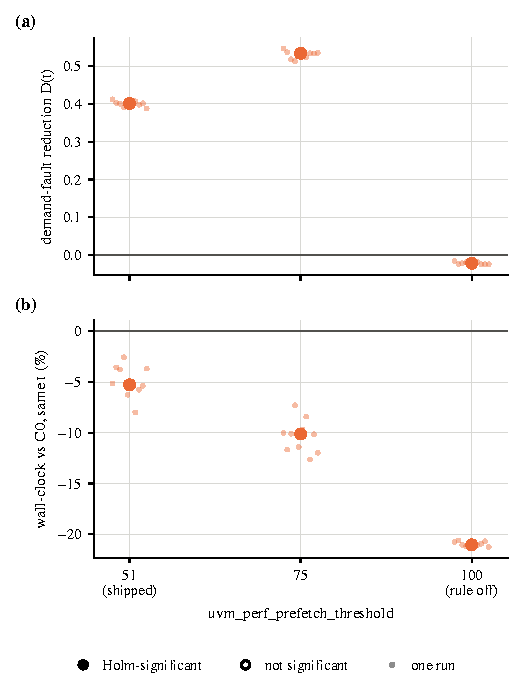
\includegraphics[width=\columnwidth]{figures/fig_e5_threshold_dose_response}
\caption{Fault reduction from staging grows with the threshold and vanishes
when the density rule is disabled (E5, Stencil-24K, C7-W512 vs C0 at each
threshold; 10 runs per cell).}
\label{fig:e5}
\end{figure}

\subsection{The Same Lever Without Speculation}
\label{sec:spec-matched}

If staging gains only by helping regions pass the threshold, lowering the
threshold should gain at least as much without staging. E6 tested this with a
second pre-registered trigger: it would fire if any stock configuration at a
lower threshold was not significantly slower than C7-W512 at 51. It fired. C0 at
threshold 0 is faster than C7-W512 at 51, which is 6.39\% slower than it; at
threshold 10 the oracle is 4.72\% slower, and at 25 the two do not differ
detectably (\texttt{E6.F1.C7W512-t51\_vs\_C0-t0}, \texttt{-t10}, \texttt{-t25}).

At matched thresholds, speculation adds little. Its gain is $-0.85\%$ at
threshold 0 and $-0.28\%$ at 10, neither significant, against minimum detectable
effects of 2.04\% and 2.28\% at the family's level, and 2.76\% at 25, which is
significant (\texttt{E6.wall.C7W512-t0\_vs\_C0-t0}, \texttt{-t10}, \texttt{-t25},
\texttt{E6.mde\_family.stencil\_wall}). Staging still removes faults at every
threshold, 5.3\% of them at 0 and 22.1\% at 25 (\texttt{E6.demand.*}), but at low
thresholds the prefetcher has already taken most regions, and the faults that
remain are too few to matter: one pre-registered expectation predicted a
wall-clock gain from the 5.3\% at threshold 0, and it failed (X4).

\begin{figure}[t]
\centering
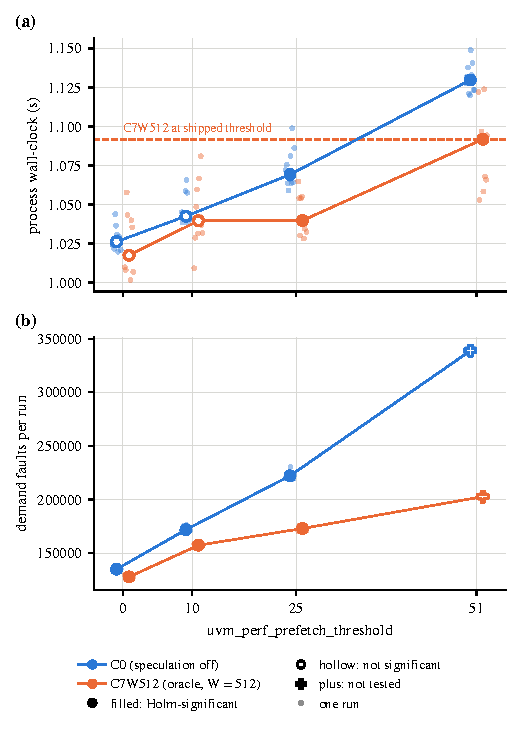
\includegraphics[width=\columnwidth]{figures/fig_e6_threshold_baseline}
\caption{C7-W512 at the shipped threshold against the stock driver at lower
thresholds, and each threshold with and without speculation (E6, Stencil-24K).}
\label{fig:e6}
\end{figure}

\subsection{What Speculation Costs on the Critical Path}
\label{sec:spec-cost}

The prediction hook runs on the servicing thread for every fault. Handing one
prediction to the worker costs 54\,ns with the prefetcher off and 75\,ns with it
on, on Stencil-24K, and 114\,ns on GraphBFS-23
(\texttt{E1b.stencil.C64096-C1}, \texttt{E1b.stencil.C74096-C0},
\texttt{E1b.graphbfs.C64096-C1}). With the original oracle the rest of the hook,
the lookup itself, cost a further 140--167\,ns per fault. The fast lookup of
Section~\ref{sec:design-oracle} removed 78--88\% of that residual
(\texttt{E3b.*.residual}): an instrument meant to bound speculation had been
paying most of speculation's per-fault cost itself (catalog entry~21).

At full width the queue is never the bottleneck: C7-W512 enqueues about 2{,}200
items per Stencil-24K run and drops none (\texttt{E4.mech.stencil.C7-W512}).

\subsection{Summary}

Off-path staging, driven by an oracle as good as the workload allows, does two
things in this driver. It moves copy work off the servicing thread, which is
worth 21--23\% only against a driver whose prefetcher is off, and it feeds the
prefetcher's density count, which is
worth 3.4--5.3\% against the shipped driver.
It prevents no fault directly. The second effect is available, and larger,
from the threshold alone; Section~\ref{sec:threshold} measures what that lever
does on its own.

% =====================================================================
% Section VII -- The Prefetch Threshold on Its Own
% SpecAsync-UVM manuscript, draft 1 (2026-11-06)
% Every number: paper/support/RESULTS_FACTS.md Section VII (evidence ids
% in the text as \texttt{} for review; strip before submission).
% Stock module 6284DA42 throughout. delta = (t - t51)/t51.
% [WL]   Family B workload names (stencil8k, sweep4k, sweep16k, stream,
%        sgemm, cufft, graphbfs, oversub) -- use the names Section V/the
%        benchmark table defines; "oversub" is the oversubscribed dense
%        stencil cell (XB3). Confirm.
% [FIG]  figure file names from RESULTS_FACTS VII(f); confirm paths.
% =====================================================================

\section{The Prefetch Threshold on Its Own}
\label{sec:threshold}

Section~\ref{sec:spec} found that speculation helps only by making regions pass
the density test sooner. This section measures the test's threshold directly,
on the unmodified driver: first on dense and streaming workloads on two GPUs,
then on a benchmark whose access density we control, then on system-allocated
memory. All comparisons are against the shipped threshold, 51.

\subsection{Dense Access: Faster at a Lower Threshold, on Two GPUs}
\label{sec:thr-dense}

On the RTX~5070~Ti, lowering the threshold to 0 makes Stencil-24K 9.57\% faster,
and to 10, 7.13\% faster (\texttt{E7.A.stencil.*}); the minimum detectable
effects are 1.23\% and 1.28\%. This was the confirmatory test of E7, run after
E6 had found the effect with our module loaded.

Table~\ref{tab:e7} gives the eight further workloads. At threshold 0, four are
significantly faster, by 2.49--16.95\%, and none is significantly slower; the
same holds at 25. The four without a significant change are short runs whose
minimum detectable effects are large, 7--12\% for three of them, so they are
not evidence of no effect; the exception is GraphBFS-23, which runs long,
changes by $-0.26\%$ and could have shown an effect of 0.86\%. The largest gain
is on a dense workload whose array exceeds GPU memory, 16.95\%; a pre-registered
expectation that oversubscription would make the low threshold slower failed
(XB3). For dense access, oversubscription does not reverse the effect.

On the Tesla~T4, with the same driver release, Stencil-24K is 5.07\% faster at
threshold 0 and 3.21\% at 10 (\texttt{T4.A.stencil.*}), and 12 of the 14 further
tests are significantly faster with none slower (\texttt{T4.B.count}). The
oversubscribed workload could not be run there, because the instance's host
memory was smaller than the array (Section~\ref{sec:protocol}). The T4's lower
run-to-run variance makes small effects significant: GraphBFS-23 is 0.14\%
faster, a significant but negligible change.

\begin{table}[t]
\centering
\footnotesize
\caption{Stock driver, threshold 0 against 51 (E7, RTX~5070~Ti).
$\delta$: change in median wall-clock; MDE at the family's level
($m = 16$). Bold: Holm-significant.}
\label{tab:e7}
\input{tables/T-E7}
\end{table}

Tracing shows where the dense gain comes from. On Stencil-24K the bytes moved to
the GPU are the same at both thresholds, within 0.74\%, but the GPU raises
27{,}876 faults at threshold 0 against 91{,}935 at 51 (\texttt{E9.ratio.stencil}).
The lower threshold does not move less data; it moves it in fewer, larger
steps. Part of the gain is not on the GPU at all. The same threshold governs
prefetching when the CPU faults on managed memory (Section~\ref{sec:bg-prefetcher}),
and in every traced run the CPU faults six times less often at threshold 0, all
of them while the host initialises the array (\texttt{E9.ratio.cpu\_faults\_t51\_over\_t0},
\texttt{E9.cpu\_phase.fill\_only}). On the dense cells of our sparse benchmark,
17--23\% of the wall-clock gain falls outside the GPU kernels
(\texttt{E8.outside\_kernels.share\_dense}).

\subsection{Sparse Access: The Lever Cuts Both Ways}
\label{sec:thr-sparse}

The dense results do not say what the low threshold costs when a program uses
only a little of each region. Our sparse benchmark touches $K$ pages per
2\,MB block, chosen at random from a fixed list, over an 8\,GiB array that fits
in GPU memory and a 24\,GiB array that does not. E8 pre-registered a trigger
that would declare the dense-access result not general if any cell with
$K < 512$ was significantly slower at a lower threshold. It fired.

\begin{table}[t]
\centering
\footnotesize
\caption{Sparse benchmark, stock driver, threshold 0 against 51 (E8). $K$:
pages touched per 2\,MB block. Bold: Holm-significant ($m = 16$).}
\label{tab:e8}
\input{tables/T-E8}
\end{table}

With the array in GPU memory the effects are small and mixed: $+3.95\%$ at
$K = 1$ and $-2.32\%$ at $K = 8$, then $-9.69\%$ and $-7.54\%$ at $K = 64$ and
512 (\texttt{E8.in.*}). Once the array exceeds GPU memory, the low threshold is
84.96\% slower at $K = 1$ and 41.15\% slower at $K = 8$, while $K = 64$ and 512
are still 9.67\% and 7.66\% faster (\texttt{E8.ov.*}). At threshold 25 the
$K = 8$ cell is 46.71\% slower and the $K = 1$ cell only 1.88\%. Two
pre-registered expectations about the shape of this pattern failed: the effect
is not monotonic in $K$ (XS4), and threshold 25 does not always lie between 0
and 51 (XS5).

\begin{figure}[t]
\centering
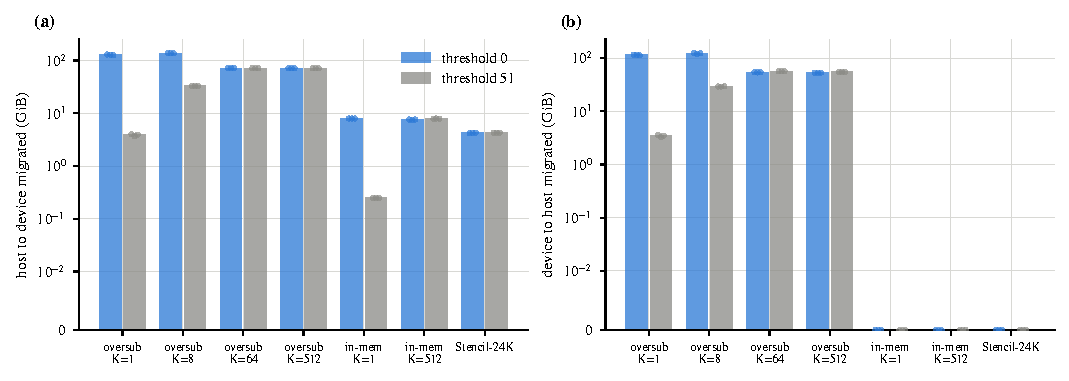
\includegraphics[width=\columnwidth]{figures/fig_e9_migrated_bytes}
\caption{Bytes migrated to and from the GPU per run, by access density and
threshold (E9, nsys, $n = 3$). Oversubscribed, $K = 1$: 129.8\,GiB at
threshold 0 against 3.96\,GiB at 51.}
\label{fig:e9}
\end{figure}

Tracing explains the slowdown (Fig.~\ref{fig:e9}). With the oversubscribed
array and $K = 1$, a run moves 129.8\,GiB to the GPU at threshold 0 and
3.96\,GiB at 51, a factor of 32.8, and almost as much back
(\texttt{E9.cell.ov\_k1.*}). At threshold 0 the first fault in each region
brings in the whole region; with one useful page per block, nearly all of it is
evicted unused and brought back on the next pass. At $K \ge 64$ the traffic is
the same at both thresholds, about 72\,GiB, because the density rule takes whole
regions at 51 too. The slowdown is on the GPU side: the time outside the kernels
falls slightly at threshold 0 even in the slowest cell
(\texttt{E8.outside\_kernels.sparse\_ov}).

\subsection{System-Allocated Memory}
\label{sec:thr-hmm}

On memory allocated with \texttt{malloc}, which the driver services through
HMM (Section~\ref{sec:bg-hmm}), we ran two further gates with arrays that fit in
GPU memory. H1 replicated the dense gain: Stencil-24K is 7.97\% faster at
threshold 0 (\texttt{H1.stencil.*}), less than on managed memory, as it should
be if part of the managed gain was the CPU-side effect above, which HMM does not
share; the two runs are different sessions, so we do not estimate that share
from them.

\begin{figure}[t]
\centering
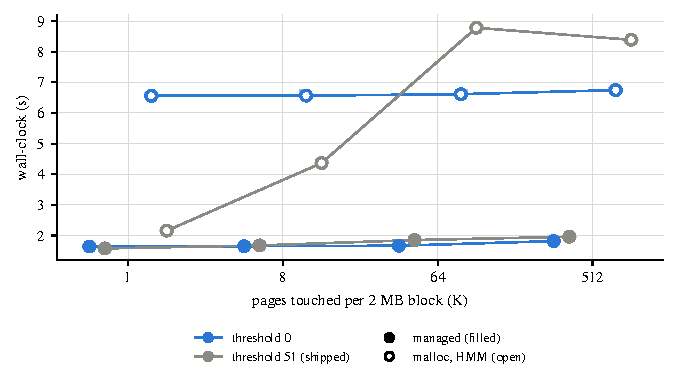
\includegraphics[width=\columnwidth]{figures/F-H2-time}
\caption{Sparse benchmark in GPU memory, by allocator and threshold (H2; 10
runs per cell). Open markers: \texttt{malloc} (HMM); filled: managed.}
\label{fig:h2}
\end{figure}

H1 also found something we had not predicted: with $K = 1$ the low threshold was
about three times slower on HMM, with no oversubscription. H2 pre-registered a
test of an explanation, stating that the hypothesis came after the observation
(Section~\ref{sec:protocol}). Fig.~\ref{fig:h2} shows the result. On HMM, the
time at threshold 0 is the same at every $K$, within 2.8\% (\texttt{H2.Z1}),
because the first fault in each region migrates all of it; at 51 it rises with
$K$. The low threshold is 203.65\% slower at $K = 1$ and 50.39\% slower at $K = 8$,
and 24.66\% and 19.56\% faster at $K = 64$ and 512 (\texttt{H2.malloc\_*}). On
managed memory, in the same session, the same cells change by $+3.92\%$,
$-1.49\%$, $-9.99\%$ and $-7.19\%$ (\texttt{H2.managed\_*}), within a point of
E8's values from an earlier session.

The volume moved does not explain the difference between the allocators. At
threshold 0 a $K = 1$ pass moves essentially the whole array on both: on HMM,
measured as GPU memory in use, 1.03 of the array (\texttt{H2.res.malloc.k1.t0});
on managed memory, measured as traced bytes in E9, 1.00 (\texttt{E9.htod\_frac.in\_k1.t0}).
At 51 the same pass moves 0.061 and 0.031 of it. The cost of moving it differs:
the $K = 1$ slowdown is 199.7 percentage points larger on HMM, with a 95\%
bootstrap interval of 198.1 to 201.7 (\texttt{H2.Z7}). This is consistent with
HMM's migration in 4\,KB units through \texttt{migrate\_vma}, against 2\,MB
chunks for managed memory (Section~\ref{sec:bg-hmm}); H2 does not isolate that
cause. One caution about the measure: on managed memory, GPU memory in use
records allocation, not migration, so we use it for HMM only (catalog
entry~31).

Two limits apply. These are in-memory results; the first oversubscribed HMM
cell crashed the stock driver, and that case was not measured
(Section~\ref{sec:protocol}). And two of H2's expectations about the shape of
the curve at threshold 51 failed (Z2, Z3): at 51, $K = 512$ is faster than
$K = 64$.

\subsection{Summary}

No fixed threshold dominates the shipped one. A low threshold helps dense and
streaming access, on two GPU generations, by moving the same data in fewer
steps and by reducing CPU faults during initialisation. It hurts sparse access
by moving data the program never uses, which costs heavily once the array
exceeds GPU memory and, on system-allocated memory, even before. This is the
trade-off Go \emph{et al.}\ reported \cite{go2023earlyadaptor}; our measurements
replicate it on newer hardware and add the access-density, traced-byte and HMM
dimensions. Section~\ref{sec:discussion} discusses what it implies for a
threshold that adapts.

% =====================================================================
% Section VIII -- A Catalog of Measurement Artifacts
% SpecAsync-UVM manuscript, draft 1 (2026-11-06)
% Source: ARTIFACT_CATALOG.md (31 entries), RESULTS_FACTS.md Section VIII
% (family counts and how-caught column), T-CAT (paper/tables/t_cat.tex).
% Entry numbers are the catalog's. The "103 days" for #13 is from the
% catalog text; confirmed in C15 (2026-06-13 to 2026-09-24).
% =====================================================================

\section{A Catalog of Measurement Artifacts}
\label{sec:pitfalls}

Over the course of this study we recorded 31 artifacts: errors in measurement,
analysis or procedure, each with the false conclusion it produced or would have
produced. We report them for two reasons.
Several of them shaped the results of Sections~\ref{sec:spec}
and~\ref{sec:threshold}, including the reversal of this study's earlier
conclusion, so a reader needs them to judge those results. And most are not
specific to our mechanism: they can arise in any measurement of a GPU driver.

\subsection{Families}

We group the entries by the mechanism of the error, not by its consequence
(Table~\ref{tab:families}).

\begin{table}[t]
\centering
\footnotesize
\caption{Catalog entries by family.}
\label{tab:families}
\begin{tabular}{@{}l l r@{}}
\toprule
Family & Entries & $n$\\
\midrule
Aggregation-level mismatch & 7, 8, 9, 13, 16, 17, 18, 25, 27 & 9\\
Validation that could not fail & 1, 2, 12, 14, 15, 31 & 6\\
Instrument cost and blindness & 4, 5, 19, 20, 21 & 5\\
Operational hazards & 3, 10, 11, 22, 24, 28, 29, 30 & 8\\
Record integrity & 23, 26 & 2\\
Uncategorised (a genuine outlier) & 6 & 1\\
\bottomrule
\end{tabular}
\end{table}

\paragraph{Aggregation-level mismatch}
A quantity is recorded at one level and consumed at another: per batch and
per fault, per trial and per run, a share of one window applied to another. The
most consequential entry in the catalog is of this kind (\#13). Our first
oracle recorded faults once per batch and replayed them once per fault, so it
ran ahead of the application and wrapped. Every oracle result for 103 days was
read as the result of a maximally favourable predictor, and the conclusion
that ``even oracle prediction yields no benefit'' was the paper's thesis. The
others in the family are smaller versions of the same error: capped ring
counts read as totals (\#7), rates computed over the wrong denominator (\#8,
\#16), a ceiling expressed in the units of a different window (\#9, \#25), and
a multiplicity correction hard-coded for a family of 16 and reused for others
(\#27, Section~\ref{sec:protocol}).

\paragraph{Validation that could not fail}
A check passes, but it would have passed whatever the truth was. The first
fix to the oracle was validated by an improvement, without an absolute
ceiling against which to judge it (\#15). A positive control that could not have
failed was read as showing that the fix, its hit accounting and the width path
were sound (\#14). A large speedup under oversubscription,
measured against a crippled baseline, appeared to reverse the paper's
conclusion (\#12). The newest entry is
of this kind too (\#31). We validated GPU memory in use as a measure of
migrated volume on HMM memory, where the driver allocates 4\,KB pages, and then
used it on managed memory, where the driver allocates a whole 2\,MB chunk per
block on the first fault. There it reads allocation, not migration, and an
expectation scored on it held (Section~\ref{sec:thr-hmm}).

\paragraph{Instrument cost and blindness}
An instrument changes what it measures, or cannot see it. The clearest case is
our oracle (\#21): its lookup ran on the fault-servicing thread under a global
lock, so an instrument meant to bound speculation's benefit was paying most of
speculation's per-fault cost (Section~\ref{sec:spec-cost}). Another counter,
named \texttt{spec\_hits}, counted faults on pages predicted within a time
window and was read as prediction success; a second counter, measuring whether
the worker actually finished first, disagreed with it (\#20). Two entries
concern our own ring buffers, read at a drifting byte offset (\#5) and in slot
order rather than time order (\#19).

\paragraph{Operational hazards}
These are errors of procedure: results taken with address randomisation
disabled read as general platform behaviour (\#10), a host memory leak (\#11), a kernel-log diff
by line count that could miss lines (\#24), a driver patch silently replaced by a Git LFS
pointer (\#28), a session ended by our own clean-up command (\#29), and an
oversubscribed run sized against GPU memory but not host memory (\#30). The one
that changed our development protocol is \#22: an instrumentation counter called
a driver helper that returns a null pointer when the GPU has no state in a
block, guarded only by a non-fatal assertion, and the kernel oopsed
(Section~\ref{sec:design-safety}).

\paragraph{Record integrity}
Two entries concern our records rather than our measurements: a platform table
that silently fell behind a driver upgrade (\#23), and a status log treated as
a primary record of timing (\#26). Section~\ref{sec:protocol} explains why we
establish the order of events by version-control ancestry, not by the clocks in
those records.

\subsection{How the Errors Were Caught}

Each entry records how it was found. Of the nine aggregation-level errors, eight
were caught only by a later, independent pass: a re-investigation, a source
audit, or the author of a later gate. Seven of them had already reached a
reported figure or conclusion. One (\#25) was caught inside the gate that made
it, by a pre-registered prediction test: E0.9b's addendum predicted, from pilot
runs, the interval in which its result should fall, and the result fell outside
it. Across all families, four errors were caught inside their own gate, and all
four by a check written before the measurement: a pre-registered test (\#10,
\#21, \#25) or a pre-registered smoke pass (\#30).

We state this pattern descriptively. The samples are small, two or three entries
per catching mechanism, and the counts are biased: an error caught inside its gate may
never have been recorded as an artifact at all, so in-gate catches are
under-counted by construction. Two lessons nevertheless shaped the protocol of
Section~\ref{sec:protocol}. A check that cannot fail is not a check, hence the
positive controls that must also reject a perturbed copy. And an error of
aggregation level is invisible from inside the analysis that makes it, because
every step is arithmetically correct; what catches it is a second, independent
path to the same number.

The full catalog, with the false conclusion and the means of detection for each
entry, is in the supplementary material (Section S3).

% =====================================================================
% Section IX -- Discussion and Conclusion
% SpecAsync-UVM manuscript, draft 1 (2026-11-06)
% No new numbers: every number below appears in Sections I, VI-VIII and
% was checked there (C14/C15). Run the C15 number check over this file.
% [BUG] The stock-driver oops is described, not cited; if the NVIDIA issue
%       is filed before submission, cite its number here.
% =====================================================================

\section{Discussion and Conclusion}
\label{sec:discussion}

\subsection{What Off-Path Staging Can Do in This Driver}

Our results answer the question we set out to test, but not in the way the
idea's proponents, including our own earlier draft, expected. Moving residency
work off the fault-servicing thread works as an engineering matter: the worker
staged 99.95\% of pages ahead of demand, and the copies it made shortened the
lock-held dispatch. It does not remove faults, because only fault service
installs mappings (Section~\ref{sec:bg-resident-mapped}). Its one route to
preventing faults runs through the prefetcher's density count, and the same
effect is available, and larger, by lowering the threshold
(Section~\ref{sec:spec-matched}).

Two ways forward follow. The first is to stage from where mapping is possible.
Explicit prefetch from user space runs the driver's make-resident-and-map path,
which is why a user-space predictor can remove faults where our worker cannot
\cite{shen2026stride}. The second is to change the driver so that a background
path may install mappings. That is a larger change than ours: mapping touches
page tables the servicing thread also writes, and would have to respect the
driver's lock order and replay protocol. We have not attempted it. Our
measurements bound what it could gain only indirectly, since Stencil-24K
already runs 9.57\% faster when the prefetcher simply maps more on each fault.

\subsection{What a Better Threshold Would Need}

No fixed threshold dominates the shipped one (Section~\ref{sec:threshold}). Go
\emph{et al.}\ drew the same conclusion and built a controller that adapts the
threshold at run time \cite{go2023earlyadaptor}. Our measurements suggest three
inputs such a controller needs. The first is the access density within a
region: on oversubscribed managed memory and on HMM, the sign of the effect changed
between 8 and 64 pages per 2\,MB block. The second is memory pressure: on managed memory
the cost of a low threshold for sparse access was small in memory and large
once the array was oversubscribed. The third is the cost of migration itself:
on system-allocated memory, which moves in 4\,KB units, the same sparse access
was much slower at a low threshold even in memory. A controller tuned on
managed memory would therefore choose wrongly for HMM. These are observations
from one synthetic benchmark at one oversubscription ratio, and they locate a
crossover only between the densities we measured.

Part of the dense-access gain lies outside the GPU. The same threshold governs
prefetching for CPU faults on managed memory, and at threshold 0 the CPU faulted
six times less often while initialising the array; on dense cells 17--23\% of
the wall-clock gain was outside the kernels. A benchmark that initialises its
data on the GPU, or with explicit copies, would see less of it.

\subsection{System-Allocated Memory and Other Vendors}

HMM lets a GPU fault on ordinary memory, and Allen \emph{et al.}\ name it as a
motivation for studying the fault path \cite{allen2024finegrain}. On NVIDIA's
open driver it shares the managed path's prefetcher and threshold but not its
migration granularity, and that difference changed the sparse-access cost by
about two hundred percentage points (Section~\ref{sec:thr-hmm}). AMD GPUs reach system
memory through the same kernel interface, and Cooper \emph{et al.}\ report the
same tension between aggressive range prefetching and access pattern on
MI250X \cite{cooper2024svm}. Whether a density-aware prefetch policy would help
there, where the driver and its prefetcher are different, is a question our
measurements raise but cannot answer.

\subsection{Threats to Validity}

\paragraph{Scope of the speculation results}
The oracle is near-perfect only for Stencil-24K, whose first-touch order varies
by about a hundred ranks between runs; for GraphBFS-23 it is a weakened oracle.
The speculation results therefore bound what off-path staging can achieve on
one regular workload and do not evaluate a practical predictor. They come from
one GPU and one driver release.

\paragraph{Scope of the threshold results}
The dense-access threshold result replicates on a second GPU generation with
the same driver release. The sparse-access, oversubscription and HMM results
come from the RTX~5070~Ti alone, from one synthetic benchmark with one fixed
page list, and from one oversubscription ratio. The HMM results are for arrays
that fit in GPU memory: the first oversubscribed HMM run crashed the stock
driver, a null-pointer dereference in its chunk-free path followed by a soft
lockup of the fault handler, with no modified code loaded. The stop rule
forbade a retry, so the case was not measured.

\paragraph{Measurement}
The outcome of record is process wall-clock, which includes CUDA
initialisation and host-side setup; we chose it because it is what a user
experiences, and we separate kernel time from the rest where it matters
(Section~\ref{sec:thr-dense}). Each cell has ten runs, and comparisons across
sessions are reported side by side but never pooled. Two of our instruments
had limits we found only after use, GPU memory in use on managed memory and
the oracle's own lookup cost; both are in the catalog
(Section~\ref{sec:pitfalls}), and no claim rests on either.

\paragraph{The study's own history}
This paper reverses an earlier version of itself. The pre-registered gates,
the positive controls and the catalog are our response, and
Section~\ref{sec:pitfalls} reports the errors they caught and those they did
not.

\subsection{Conclusion}

We built off-path page staging into NVIDIA's open-source UVM driver and
measured it, with an oracle, under pre-registered tests. Staging cannot prevent
a fault, because in this driver only fault service maps a page. Against the
shipped driver it helps, by 3.4--5.3\% on a regular workload, only by raising
the count in the prefetcher's density rule, and lowering that rule's threshold
does more without any speculation. The threshold itself cuts both ways: it
speeds up dense access on two GPU generations and slows sparse access, under
memory pressure on managed memory and even without it on system-allocated
memory. For anyone building on the UVM fault path, the practical lesson is that
the lever worth adapting is the one the driver already has, and that the input
it most needs is how densely each region is used.


% Generated table fragments (paper/tables/, see TABLES.md) are \input by the
% section that uses them, for example \begin{tabular}{@{}llrrrrrcr@{}}
\toprule
Workload & Arm vs C0 & Median C0 (s) & Median arm (s) & $\Delta$ (\%) & MWU $p$ & Holm thr. & Sig. & MDE, $\alpha/18$ (s) \\
\midrule
Stencil-24K & C7-W1 (F1) & 1.1295 & 1.1958 & +5.87 & 1.08e-5 & 0.0028 & yes & 0.0266 \\ % E4.F1.stencil.C7-W1_vs_C0
 & C7-W64 (F1) & 1.1295 & 1.1089 & $-$1.83 & 8.92e-2 & 0.0071 & no & 0.0274 \\ % E4.F1.stencil.C7-W64_vs_C0
 & C7-W512 (F1) & 1.1295 & 1.0738 & $-$4.93 & 1.08e-5 & 0.0029 & yes & 0.0197 \\ % E4.F1.stencil.C7-W512_vs_C0
 & C6-W512 (F4) & 1.1295 & 3.2975 & +191.95 & 1.08e-5 & 0.0042 & yes & 0.0252 \\ % E4.F4.stencil.C6-W512_vs_C0
\midrule
GraphBFS-23 & C7-W1 (F1) & 31.5513 & 31.4619 & $-$0.28 & 3.53e-1 & 0.0125 & no & 0.1848 \\ % E4.F1.graphbfs.C7-W1_vs_C0
 & C7-W64 (F1) & 31.5513 & 31.5199 & $-$0.10 & 4.81e-1 & 0.0250 & no & 0.1810 \\ % E4.F1.graphbfs.C7-W64_vs_C0
 & C7-W512 (F1) & 31.5513 & 31.5322 & $-$0.06 & 5.29e-1 & 0.0500 & no & 0.1194 \\ % E4.F1.graphbfs.C7-W512_vs_C0
 & C6-W512 (F4) & 31.5513 & 32.7692 & +3.86 & 1.08e-5 & 0.0050 & yes & 0.1641 \\ % E4.F4.graphbfs.C6-W512_vs_C0
\bottomrule
\end{tabular}
.

\bibliographystyle{IEEEtran}
\bibliography{ref}

\end{document}
